\documentclass[a4paper,10pt]{article} \usepackage[utf8]{inputenc}
\usepackage[hidelinks]{hyperref} \def\UrlBreaks{\do\/\do-} % breaks long url in
% references
\usepackage{graphicx} \usepackage[english]{babel} \usepackage{listings}
\usepackage{cite} \usepackage{tikz}
\usepackage[labelfont=it,
textfont={it},singlelinecheck=on,justification=centering]{caption}
\usepackage{amsmath} \usepackage{float} \usepackage{xcolor}
\usepackage{comment}

\lstset{basicstyle=\ttfamily\footnotesize,breaklines=true} \lstset{numbers=left,
numberstyle=\tiny, stepnumber=1, numbersep=5pt} \lstset{language=TeX}
\setlength{\parskip}{1em} \renewcommand{\baselinestretch}{1.2}
\newcommand{\x}[1]{{\tt #1}} \newcommand{\code}[1]{{\tt #1}}
\newcommand{\todo}[1]{{\color{red} TODO #1 }}
\newcommand{\bs}[1]{{\color{red}#1}}

\title{\textbf{Storj\\A Decentralized Cloud Storage Network Framework}}
\author{\\ \parbox{\linewidth}{\centering\small Alex Bender (bender@storj.io),
Alex Leitner (alex@storj.io),\\ Benjamin Sirb (bens@storj.io), Braydon Fuller
(braydon@storj.io),\\ Bryan White (bryan@storj.io), Chris Pollard
(cpollard1001@gmail.com),\\ Dennis Coyle (dennis@storj.io), Dylan Lott
(dylan@storj.io),\\ Garrett Ransom (garrett@storj.io), Gordon Hall
(gordonhall@openmailbox.org),\\ James Hagans (jhagans@storj.io), James 
Prestwich (james@storj.io),\\ John Gleeson (jg@storj.io), Josh Brandoff
(josh@brandoff.is), JT Olio (jt@storj.io),\\ Kaloyan Raev (kaloyan@storj.io),
Kishore Aligeti (kishore@storj.io),\\ Nadine Farah (nadine@storj.io), Natalie
Villasana (nat@storj.io),\\ Patrick Gerbes (patrick@storj.io), Philip Hutchins
(philip@storj.io),\\ Shawn Wilkinson (shawn@storj.io), Tome Boshevski
(tome@storj.io)}\\\\\small \url{https://github.com/storj/whitepaper} }\date
{v3.0, June 24, 2018}

\begin{document}

\maketitle

\begin{abstract}
\begin{tikzpicture}[remember picture,overlay]
\node[rotate=45,scale=15,text opacity=0.1]
at (current page.center) {DRAFT};
\end{tikzpicture}

Decentralized Cloud Storage represents a fundamental shift in
the efficiency and economics of distributed storage.
Eliminating central control allows users to store and share data
without reliance on a third-party storage provider. Decentralization mitigates
many traditional data failures and outages while simultaneously increasing
security and privacy. At a greater rate than any single entity can afford, it 
allows market forces to innovate on cheaper ways to provide storage. 
While there are many ways to build such a system, there are some specific 
responsibilities any given system should address. 
Based on our experience with petabyte-scale
storage systems, we introduce a modular framework for considering these
responsibilities and building such a system. Additionally, we describe initial 
concrete implementations for each responsibility of the framework. 
\end{abstract}

\todo{
Remaining big todo items:
\begin{itemize}
\item Settle on a choice for what $n,k,r,C,K$ etc. mean in reference to the 
network. (Different variables are being used to represent the same thing.)
\item Datascience: write an appendix about repair bandwidth based on node
  churn and uptime
\item Datascience: Write an appendix about how we select RS numbers
\item Eng/marketing: Quality control/branding section - talk about how we
  plan to ensure satellite quality by quality control evaluations, formal
  partnerships, relationships, and not letting poor quality satellites
  use the brand.
\end{itemize}

Remaining medium todo items:
\begin{itemize}
\item Anyone: Make sure this paper explains conclusively why we're doing v3 and
  why we won't have to do a v4 - difference between framework vs concrete
  sections
\item Anyone:
  Clean up distributed consensus positioning in the Metadata section.
\item JT: Move merkle-tree-based-filesystem idea to future work section
\item Eng: Describe how path encryption works
\item Eng: Describe payer (satellite) ids and why they're needed
\item Eng: General data repair framework description
\item Anyone: Clean up attacks section
\item Anyone: Clean up selected calculations section
\item Eng: more macaroon details
\end{itemize}

Remaining little todo items:
\begin{itemize}
\item Anyone: Write the security and privacy requirements section
\item Eng: Write a future work section about eliminating TLS handshakes
\item Anyone: Clean up the pacing for the structured file storage section
\item Eng: Write about how piece ids are generated
\item Eng: Describe pointers
\item Eng: Future work section about reputation sharing
\item Eng: Future work section about finding a better data structure than
 a bloom filter for gc
\item Once this is all done, look through to ensure no orphaned lines, 
section headings, etc.
\end{itemize}
}

\section{Introduction}

Storj is a protocol that creates a distributed network for the reliable storage
of data and facilitates payment for successful data storage and transfer
between peers.
The Storj protocol enables peers on the network to transfer and receive data,
verify the integrity and availability of remote data, and pay other nodes
for storing data.
While not all peers in the network have the same responsibilities,
the goal is for every peer to be an autonomous agent, capable of performing
these actions with little to no significant human interaction.


There are a handful of storage-based companies emerging that aim to create vast networks to store data. 
Companies such as Wuala, Allmydata, Tahoe-LAFS, Space Monkey, Sia, Maidsafe, Filecoin, Crashplan, Mozy, HDFS, 
Storj, S3, GFS,  and others believe that a single computer is not as powerful or secure as these networks. One advantage of 
building large networks is that it increases security in how data is being stored. As more people enter the network, it becomes more challenging to steal data.  While all these companies share a common core of building robust and secure networks, they also share common principles of how it can be achieved. Companies generate redundancy for data in case of failure, store this redundancy in locations with varying degrees of failure isolation, and then keep track of where the data was placed. However, the technical implementations, designs, and other considerations greatly vary with each company. 

When designing a distributed storage system, there are multitude of optimizations that can be made: speed, capacity, trustlessness, byzantine fault tolerance, cost, etc. Unlike optimizing cost or speed, data needs to be persistent throughout the network with no loss. One way of achieving this is having nodes communicate with each other and creating a functional systems that are seamlessly integrated to store and retrieve data. 

We propose a framework that will horizontally scale to serve data to hundreds of millions of people across the world. Our system, The Storj Network, is a robust object store that encrypts, shards, and sends data to our global community for storage.  Data is served with low latency and purposefully designed to prevent breaches that have continuously plagued companies. In order to accomplish this task, we've designed our system to be independent components with task-specific jobs.  We've integrated these components with each other to perform a secure, robust, and reliable storage system.

The rest of the paper is divided into 4
sections. In Section \ref{sec:design_constraints}, we discuss the design space
in which Storj operates in and elaborate on specific design constraints that
focus what we plan to optimize for.
Section \ref{sec:framework} covers our framework and proposes a simple
concrete implementation of each component.
Section \ref{sec:product_details} covers specific details
about how we will deliver this implementation to users. Section
\ref{sec:future_work} covers future areas of research.

\section{Storj design constraints and
considerations}\label{sec:design_constraints}

Before designing a system, it's important to understand its requirements.
We will begin with a discussion of Storj's design constraints.

\subsection{S3 compatibility}

The flagship cloud storage product is Amazon's Simple Storage Service, or S3 for
short. Most cloud storage products provide some form of compatibility with the
S3 API.

Until a decentralized cloud storage protocol is the {\em lingua franca} of
storage protocols, we must create a graceful transition from centralized providers. 
This will alleviate any switching costs for users with data currently stored on 
a centralized provider.  Our objective is for Storj to compete successfully in the wider cloud storage 
industry and bring decentralized cloud storage into the mainstream, enabling 
more people greater security and less centralized control. To achieve this, 
applications built against S3 should be configurable to work with Storj with 
minimal friction and changes. Imagine if 90\% of existing application services 
could switch to Storj with a
single configuration change. \todo{maybe talk about s3 market penetration?} 
This adds strong requirements on feature set, performance, and durability.

\subsection{Device failure and churn}

For any storage system, but especially a distributed storage system, component
failure is a guarantee. All hard drives fail after enough wear
\cite{backblaze-hd-2018-q1}, and the servers providing network access to
these hard drives will eventually fail, too. Network links die, power is lost,
and storage mediums become unreliable. \todo{Maybe add a joke about some ridiculous failure case here}  For data to outlast individual component
failure, data must be stored with enough redundancy to recover from failure.
Perhaps more importantly, no data should be assumed to be stationary and all
data must eventually be moved. In such an environment, redundancy, data
maintanance, repair, and replacement of lost redundancy are facts of life, and
the system must account for these issues.

Decentralized systems are additionally susceptible to high churn rates, where
potential participants join the network and then leave for various reasons, well
before their hardware has actually failed. A network with a high churn rate will
use a large amount of bandwidth just to ensure durability of the data, and such
a network will fail to scale. As a result, a scalable, highly durable storage
system must prefer stable nodes and endeavor to keep the churn rate as low as
possible.

Despite the chance of hardware failure, Maymounkov et al. found that in
decentralized systems, the probability of a node staying on
for an additional hour as a member of the network is an {\em increasing}
function of uptime \cite{kad}. In other words, the longer a node is a
participant in the network, the more likely it is to continue
participating. This gives our system a strong incentive to prefer long-lived,
stable nodes.

See Appendix \ref{appendix:RS} for a discussion about how repair bandwidth varies as a
function of node churn.

\subsection{Latency}

Decentralized, distributed storage has the potential to capitalize on massive 
opportunities for parallelism in transfer rates, processing, 
and a number of other factors. Parallelism by
itself is a great way to increase overall throughput even when individual
network links are slow. However, parallelism cannot by itself improve {\em
latency}. If an individual network link has fixed latency and is a required part
of an operation, the latency of the overall operation will be bound from below
by the latency of the required network link. Therefore, a distributed system
intended for high performance applications must aggressively optimize for low
latency, both at the individual process scale and at the overall architecture
scale.

We emphasize an architectural strategy aimed at achieving low latency by
focusing on eliminating the need to wait for long tails \cite{tail-at-scale}. 
The goal is a protocol that allows for every request to be satisfiable by the
fastest nodes participating in any given transaction, without needing to wait 
for a slow subset. 
Focusing on operations where the result is only dependent on the fastest
nodes turns what could be a potential liability (highly variable performance
from individual actors) into a great source of strength for a distributed
storage network.

\subsection{Bandwidth}

Global bandwidth availability is increasing year over year; however, access to
high-bandwidth internet connections is unevenly distributed. While users in some
countries can easily access symmetric, high-speed, unlimited bandwidth, users in
other countries may have significant difficulty in obtaining access to the same.
In the United States, the way many residential internet service providers provide
internet presents two specific challenges for designers of a
decentralized network protocol. The first challenge is that the internet
connection is often asymmetric. Customers subscribe to internet service
based on an advertised download speed, but the upload speed is potentially an
order of magnitude or two slower. The second challenge is that bandwidth is
sometimes "capped" at a fixed amount of traffic per month. For example, in many
markets, Comcast poses a one terabyte per month bandwidth cap with stiff fines
for customers who go over. Such caps impose
significant limitations on the bandwidth available at any given moment.
For example,
an internet connection with a throughput of 10 MB/s and a cap of 1
TB/month cannot average more than 385 KB/s over the month without going
over the monthly bandwidth cap.

With device failure and churn guaranteed, any decentralized system will have a
corresponding amount of repair traffic. It is therefore important to make sure
there is enough headroom for the bandwidth required by data maintenance, over
and above that required for data storage and retrieval. Designing a
storage system that is careless with bandwidth usage would be to relegate that
system below storage providers with access to unlimited high-speed bandwidth,
recentralizing the system to some degree. To keep the storage system as
decentralized as possible and for it to work in as many environments as
possible, bandwidth usage must be aggressively minimized.

Please see Appendix \todo{} for a discussion on how available bandwidth,
combined with required repair traffic, limits usable space.

\subsection{Security and privacy}

\todo{we want to make sure users' data privacy is protected}

\subsection{Object size}

Broadly, large storage systems can be classified into two groups by average
object size. When storing lots of small bits of information, generally a
database is the preferred route. On the other hand, when storing lots of large
files, an object store or filesystem is ideal. We classify a "large" file as a
few megabytes or greater.

The initial product offering by Storj Labs is designed to function primarily as
an object store for larger files. While future improvements may enable
database-like use cases, the predominant use case described by this paper is
object storage. Protocol design decisions are made with the assumption that the
vast majority of objects stored will be a couple of megabytes or more. It is
worth pointing out that this will not negatively impact use cases that require
lots of files smaller than a megabyte. Such cases can admit a packing
strategy, where many small files are aggregated and stored together as one large
file. As the protocol has streaming support, small files can be retrieved
without requiring full retrieval of any aggregated object they were packed into.

\subsection{Byzantine Fault Tolerance}

Unlike datacenter-based solutions like Amazon S3, Storj operates in an untrusted
environment, where individual storage providers are not necessarily assumed to be
trustworthy. Storj operates over the public internet, and allows anyone to sign
up to become a storage provider.

We adopt the BAR (Byzantine, Altruistic, Rational) model \cite{bar} to discuss
participants in the network.
{\em Byzantine} nodes may deviate arbitrarily from the suggested protocol for
any reason. Some examples include nodes that are broken, nodes that are
trying to cheat the suggested protocol to their advantage, or nodes that
are actively trying to sabotage the protocol. In general, a Byzantine node is
one that optimizes for a utility function that is independent of the one
given for the suggested protocol.
Inevitable hardware failure aside, {\em Altruistic} nodes
participate in a proposed protocol even if the rational choice is to deviate.
{\em Rational} nodes participate exactly when it is in their net benefit to do
so, and may depart for the same reason.

Some distributed storage systems (e.g., Amazon S3) operate in an environment
where all nodes are altruistic {\color{red}add citation?}.
Storj operates in an environment where a
majority of storage nodes are rational and a minority are byzantine. Storj
assumes no altruistic nodes. Any
potential design must account for this distinction.

\section{Framework and concrete implementation}\label{sec:framework}

At a high level, there are three major operations in the system: storing data,
retrieving data, and maintaining data.

\begin{description}

\item[Storing data] When data is stored with the network, the client encrypts
it and breaks it up into multiple little pieces. It then distributes the pieces 
to peers in the network and generates and stores some metadata about where to find the data
again.

\item[Retrieving data] When data is retrieved from the network, 
the client first recovers the metadata about where to find the pieces. 
Then the pieces are retrieved and the original data is reconstructed 
on the client's local machine.

\item[Maintaining data] Data is maintained in the network with nodes replacing
missing pieces when the amount of redundancy drops below a certain threshold.
The data is reconstructed, and the missing pieces are regenerated and replaced.

\end{description}

To make this system feasible while satisfying our design constraints, we will
need to solve a number of complex challenges. Inspired by Raft \cite{raft}, we
break up the design into a collection of relatively independent concerns and
then combine them to form the desired protocol. One benefit from this approach
is that it makes 
updating individual components much easier without having to rearchitect the rest 
of the network. The individual components are:

\begin{enumerate}
\item Storage nodes
\item Peer-to-peer communication
\item Overlay network
\item Redundancy
\item Structured file storage
\item Metadata
\item Encryption
\item Authorization
\item Audits
\item Data repair
\item Storage node reputation
\item Payments
\item Payer reputation
\item Garbage collection
\end{enumerate}

\subsection{Storage nodes}

The most fundamental part of this network is the storage node.  The storage node's role is to store and return data.  Aside from storing data,
nodes should provide reliable storage space, network bandwidth, and appropriate responsiveness. In return, nodes are rewarded
for their participation. Nodes are awarded points based on how they do in certain categories. In short, storage nodes are selected to store data based on various criteria:  ping time, latency, throughput, disk space, geographic location, etc. This means that node selection almost certainly must be an explicit process.

\subsubsection{Concrete implementation}

Storage nodes will support three methods: \code{get}, \code{put}, and
\code{delete}. They store {\em pieces} (to be described in more detail
later \bs{where? reference}). Each method will take a {\em piece ID}, a 
{\em payer ID} and signature
by the payer, an optional TTL, and the other metadata required by the bandwidth
allocation protocol (also to be described later \bs{where? add section reference}).

The \code{put} operation will take a stream of bytes and store the bytes such
that any subrange of bytes can be retrieved again via a \code{get} operation.
\code{get} operations are expected to work until the TTL expires (if a TTL was
provided), or until a \code{delete} operation is received, whichever comes
first.

The {\em payer ID} forms a namespace. An identical {\em piece ID} with a
different {\em payer ID} refers to a different {\em piece}.

Storage nodes should allow administrators to configure maximum allowed disk
space usage and maximum allowed bandwidth usage over the last rolling 30 days. They should keep track of how much is remaining of both, and reject operations that do not have a valid signature
 from the appropriate payer.

\subsection{Peer-to-peer communication}

All peers on the network will need to communicate via a ubiquitous protocol. The framework requires all 
nodes to fulfill these requirements for communication: 

\begin{itemize}
\item provides peer reachability, even in the face of firewalls
and NATs. This may require techniques like STUN, relays, etc.
\item provides authentication, where each participant knows
exactly the identity of the peer with whom they are speaking.
\item provides privacy, where only the two peers
know what transfers between them.
\end{itemize}

\subsubsection{Concrete implementation}

Initially, we'll be using gRPC \cite{grpc} on top of TLS on top of $\mu$TP
\cite{utp} with added STUN functionality. Over time, we'll be replacing TLS to
reduce round trips due to connection handshakes in situations where the data is
already encrypted and forward secrecy isn't necessary. \todo{} See the Future
Work section for more details. Gateways will be provided that allow for more
standard protocols such as HTTPS.

As in S/Kademlia \cite{skad}, the {\em node ID} will be the hash of a public key
and will serve as a proof of work for joining the network. Unlike Bitcoin proof
of work \cite{bitcoin}, the work will be dependent on how many {\em trailing}
zero bits one can find in the hash output. This means that the node ID will
still be usable in a balanced Kademlia \cite{kad} tree.

Each node will operate its own certificate authority, which requires a
public/private keypair and a self-signed certificate. The certificate authority
should ideally be kept in cold storage to prevent key loss.

Each node will also have revokable leaf key pair and certificate, signed by
the node's certificate authority. Nodes will use this leaf keypair for actual
communication. Should the leaf become compromised, the node can issue a new
leaf and a new entry in a certificate revocation list.

The {\em node ID} will be determined from the certificate authority
by hashing the DER-encoded public key Pu.

\begin{equation}
\text{NodeID} = \text{SHA256}(\text{Pu})
\end{equation}

It's important that the certificate authority private key be managed with good
operational security as key rotation for the certificate authority will require
a brand new node ID.

\todo {Equation for PoW on public key, and more explanation.}

When using TLS, every peer can ascertain the ID of the node with which it is
speaking by validating the certificate chain and hashing its peer's
certificate authority's public key. It can then be estimated how much work went
into constructing the node ID by considering the number of 0 bits at the end of
the ID.

For the few cases where a node cannot achieve a successful hole punch through a
NAT or firewall via STUN, uPnP, NATPmP, or a similar technique, manual
intervention and port forwarding will be required.

\subsection{Overlay network}
The framework requires a way to look up peer network addresses by node ID
so that, given a peer's network address, any other peer can connect to it.
An {\em overlay network} can be built on top of our peer-to-peer
communication component that provides functionality similar to DNS, where a
node's ID can be resolved to an ephemeral network address for communication.

\subsubsection{Concrete implementation}

The Kademlia DHT serves as a key-value store with a built-in node lookup
protocol. We utilize this protocol to achieve DNS-like functionality for node
lookup, while ignoring the storage aspects of the Kademlia protocol due to some
issues around value republishing and limits to network growth rate, among 
other things \bs{should we provide a reference here to other potential issues 
with the Kad protocol?}.
However, using a DHT will make it difficult to achieve millisecond-level
response times when multiple DHT lookups must happen for every operation, so
more work is necessary to achieve our performance goals. Fortunately, caching
address information for an entire network of 80k nodes (for example) can be done
with 3MB of memory, so the DHT can be sped up with some simple, optional
caching.

Because a cache of the DHT can be untrusted (and peer-to-peer communication is
authenticated to avoid man-in-the-middle-attacks anyway \bs{what does this have 
to do with the fact that a DHT cache can be untrusted?}), some well-known
community-run DHT caches can be provided that simply attempt to talk to every
storage node every so often, such as every hour, evicting nodes from their
cache that have not been seen recently.
Since nodes are expected to be long lived with good uptime, they
are expected to have stable addresses that don't change often on the order of
more than once an hour. \todo{How do we handle dynamic ips in general?} Thus, such a cache will add a massive performance boost, even when slightly stale.
In addition, the protocol will be resilient against an expected degree of node
churn, so having a small number of stale addresses in a DHT cache will not alter
the expected performance of the network. Furthermore, we avoid a number of known
attacks by using the S/Kademlia extensions. \cite{skad}

\todo{talk about how we're using kademlia to advertise disk space and bandwidth
availability, and then storing that information in the cache}

\subsection{Redundancy}

At any moment, any storage node could go offline permanently. Our redundancy
strategy must store data in a way that provides access to the data with high
probability, even though any given number of individual nodes may be offline. To
achieve a certain level of {\em durability} (the probability that data will
remain available in the face of failures), many products in this space use
simple replication. Unfortunately, this ties durability to the network {\em
expansion factor}, which is the storage overhead for reliably storing data.

As an example, suppose a certain desired level of durability requires a
replication strategy that makes eight copies of the data. This yields an
expansion factor of 8x, or 800\%. This data then needs to be stored on the
network, using bandwidth in the process. Thus, more replication results in more
bandwidth usage for a fixed amount of data. As discussed in the protocol design
constraints, high bandwidth usage prevents scaling, so this is an undesireable
strategy for ensuring a high degree of file durability. Instead, {\em erasure
codes} are a more general and flexible scheme for manipulating data
durability without tying it to bandwidth usage. Importantly, erasure codes allow
changes in durability without changes in expansion factor!

An erasure code is often described by two numbers, $k$ and $n$. If a block of
data is encoded with a $(k,n)$ erasure code, there are $n$ total generated {\em
erasure shares}, where only any $k$ of them are required to recover the original
block of data. If a block of data is $s$ bytes, each of the $n$ erasure shares
is roughly $s/k$ bytes. Besides the case when $k=1$ (replication), all erasure
shares are unique. Interestingly, the durability of a $(k=20,n=40)$ erasure code
is better than a $(k=10,n=20)$ erasure code, even though the expansion factor
(2x) is the same for both! Intuitively, this is because the risk is spread
across more nodes in the $(k=20,n=40)$ case. These considerations make erasure
codes an important part of our general framework.

\begin{comment}

With the simplifying assumption that every node has an equal probability of
failure $p$, one can gain more intuition by modeling file durability as the CDF
of the binomial distribution, as seen in Equation \eqref{eq:binom_cdf}. In this
case, $P(D)$ represents the probability that at most $n-k$ erasure shares are
lost for a given file, so that $n-(n-k)=k$ erasure shares of the file remain;
i.e. the file can still be rebuilt. The CDF of the binomial distribution is
given by:

\begin{equation} P(D) = \sum_{i=0}^{n-k} \binom{n}{i} p^i
(1-p)^{n-i}\label{eq:binom_cdf}
\end{equation}
\end{comment}



With the simplifying assumption that $p$ is the monthly node 
birth/death rate (the proportion that describes the number of nodes
leaving/joining the network per month), we can model file durability 
as the CDF of the Poisson distribution with mean $\lambda=pn$, 
where we expect $\lambda$ pieces of the file to be lost monthly. To estimate 
durability, we consider the CDF up to $n-k$, 
looking at the probability that at most $n-k$ pieces 
of the file are lost in a month and the file can still be rebuilt.
The CDF is given by:
\begin{equation} 
P(D) = e^{-\lambda} \sum_{i=0}^{n-k} \frac{\lambda^i}{i!}.
\label{eq:poiss_cdf}
\end{equation}
By being able to tweak the durability independently of the expansion factor,
very high durabilities can be achieved with surprisingly low expansion factors.
Because of how limited bandwidth is as a resource, eliminating replication as a
strategy entirely and using erasure codes only for redundancy causes a drastic
decrease in bandwidth footprint and a drastic increase in the funds available
per byte on storage nodes.


\begin{table}[h]
\centering
\begin{tabular}{c c c l}
$k$ & $n$ & Exp. factor & P(D) \\
\hline 2 & 4 & 2 & 99.207366813274616391\%\\
4 & 8 & 2 & 99.858868985411326445\%\\
8 & 16 & 2 & 99.995462406878260756\%\\
16 & 32 & 2 & 99.999994620652776179\%\\
32 & 64 & 2 & 99.999999999990544376\%\\
\end{tabular}
\caption{$P(D)$ for various choices of $k$ and $n$, assuming $p=0.1$.}
\end{table}

\begin{figure} \centering
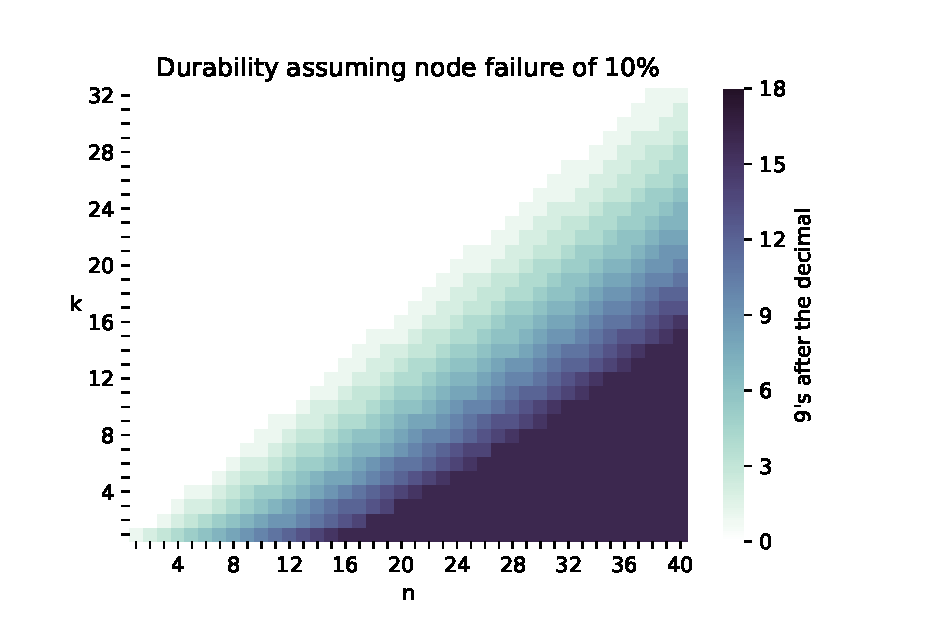
\includegraphics[width=\linewidth]{durability/durability.eps}
\label{fig:durability}
\end{figure}


\subsubsection{Streaming}

Erasure codes are used in many streaming contexts such as audio CDs and
satellite communications, so it's important to point out that using erasure
coding in general does not make our streaming design requirement more
challenging. Whatever erasure code is chosen for our framework, streaming can be
added on top by encoding small portions at a time, instead of attempting to
encode a file all at once. See the structured file storage section for more
details. \bs{add reference to the section}

\subsubsection{Long tails}

Erasure codes enable an enormous performance benefit, which is the ability to
avoid waiting for long-tail response times \cite{tail-at-scale}. For uploads, a
file can be encoded to a higher $(k, n)$ ratio than necessary for desired 
durability
guarantees. During an upload, after enough pieces have uploaded to gain required
redundancy, the remaining additional uploads can be cancelled, allowing the
upload to be blocked\bs{(?)} by the fastest nodes in a set, instead of waiting for the
slowest nodes. Downloads are similarly improved. Since more redundancy exists
than is needed, downloads can be served from the fastest peers, eliminating a
wait for temporarily slow or offline peers.

\subsubsection{Concrete implementation}

We use the Reed-Solomon erasure code \cite{rs}. For each object that we store
we choose 4 numbers, $k$, $m$, $o$, and $n$, such that $k\le m\le o\le n$.
$k$ and $n$ are the standard Reed Solomon numbers, where $k$ is the minimum
required number of pieces for reconstruction, and $n$ is the total number of
pieces generated during creation.

$m$ and $o$ are the {\em minimum safe} and {\em optimal} values, respectively.
$m$ is chosen such that if the amount of available pieces falls below $m$, a
repair is triggered immediately in an attempt to make sure we always maintain
$k$ or more pieces. $o$ is chosen such that during uploads, as soon as $o$
pieces have finished uploading, remaining pieces up to $n$ are canceled as
described above. $o$ is chosen such that storing $o$ pieces is all that is
needed to achieve the desired durability goals; $n$ is thus chosen such that
storing $n$ pieces would be excess durability.

Our durability story does not end with our selection of these numbers.
Please see section \ref{sec:data_repair} for a discussion about how we repair
data as its durability drops over time.

See Appendix \ref{appendix:RS} for how we select our Reed-Solomon numbers.

\subsection{Structured file storage}

Our design constraints include S3 compatibility. This means we should support
hierarchical objects (paths with prefixes), object metadata, arbitrarily large
files, arbitrarily large amounts of files, and so on. Similarly, our design
constraints require total security, so any such metadata will be encrypted.

Provided we have an efficient way to store data, we can build many of these
features on top our desired protocol by means of an {\em injective embedding} 
(here used in the mathematical sense). 
In other words, adding this functionality can be done by
building on top of the basic components we have already created without loss of
generality.

Because so much here depends on concrete
implementation details, our framework is described in more general terms, while our concrete implementation has significant detail.

\subsubsection{Concrete implementation}

\todo{an introduction before diving into a list of definitions}

\begin{description}
\item[Client] A user that would like to upload or download data from the network. 

\item[Bucket] A \x{bucket} is an unbounded but named
collection of \x{file}s identified by \x{path}s. Each \x{path} represents one
\x{file}, and every \x{file} has a unique \x{path}.

\item[Path] A \x{path} is a unique identifier for a \x{file} within a
\x{bucket}. A \x{path} is a string of UTF8 codepoints that begins with a forward
slash and ends with something besides a forward slash. More than one forward
slash (referred to as the \x{path separator}) separate \x{path components}.

An example path might be \code{/etc/hosts}, where the \x{path components} are
\code{etc} and \code{hosts}.

We encrypt \x{paths} before they ever leave the customer's application's
computer.

\item[File] A \x{file} is a collection of \x{stream}s. Every \x{file} has
exactly one default \x{stream} and may have 0 or more named \x{stream}s.
Multiple \x{stream}s allow flexible support of extended attributes, alternate
data streams, resource forks, and other slightly more esoteric filesystem
features.

Like \x{path}s, the data contained in a \x{file} is encrypted before it ever
leaves the client computer.

\item[Stream] A \x{stream} is an ordered collection of 0 or more \x{segment}s.
\x{segment}s have a fixed maximum size, and so the more bytes the \x{stream}
represents through \x{segment}s, the more \x{segment}s there are.

\item[Segment] A \x{segment} represents a single array of bytes, between 0 and a
user-configurable maximum \x{segment} size. Breaking large \x{file}s into
multiple \x{segment}s provides a number of security and scalability advantages.

\item[Inline Segment] An \x{inline segment} is a \x{segment} that is small
enough it makes sense to store it "inline" with the metadata that keeps track of
it, such as a \x{pointer}.

\item[Remote Segment] A \x{remote segment} is a larger \x{segment} that will be
encoded and distributed across the network. A \x{remote segment} is larger than
the metadata required to keep track of its book keeping.

\item[Stripe] A \x{stripe} is a further subdivision of a \x{segment}. A
\x{stripe} is a fixed amount of bytes that is used as an encryption and erasure
encoding boundary size. Erasure encoding happen on \x{stripe}s individually,
whereas encryption may happen on a small multiple of stripes at a time. All
\x{segments} are encrypted, but only \x{remote segments} are erasure encoded.

\item[Erasure Share] When a \x{segment} is a \x{remote segment}, its \x{stripe}s
will get erasure encoded. When a \x{stripe} is erasure encoded, it generates
multiple pieces called \x{erasure share}s. Only a subset of the \x{erasure
share}s are needed to recover the original \x{stripe}, but each \x{erasure
share} has an index identifying which \x{erasure share} it is (e.g., the first,
the second, etc.).

\item[Piece] When a \x{remote segment}'s \x{stripe}s are erasure encoded into
\x{erasure share}s, the \x{erasure share}s for that \x{remote segment} with the
same index are concatenated together, and that concatenated group of \x{erasure
share}s is called a \x{piece}. If there are $n$ \x{erasure share}s after erasure
encoding a \x{stripe}, there are $n$ \x{piece}s after processing a \x{remote
segment}. The $i$th \x{piece} is the concatenation of all of the $i$th
\x{erasure shares} from that \x{segment}'s \x{stripe}s.

\item[Piece Storage Node] A node in the network that is responsible for storing
\x{piece}s. These are operated by \x{storage node}s.

\item[Storage node] A person or group that is responsible for running and 
maintaining
\x{piece storage nodes}.

\item[Pointer] A \x{pointer} is a data structure that keeps track of which
\x{piece storage nodes} a \x{remote segment} was stored on, or the \x{inline
segment} data directly if applicable.

\todo{maybe add a diagram of how these parts relate to each other?}

\end{description}

\subsubsection{Files as Streams}

Many applications benefit from being able to keep metadata alongside files. For
example, NTFS supports "alternate data streams" for each file, HFS supports
resource forks, EXT4 supports "extended attributes," and more importantly for
our purposes, AWS S3 supports "object metadata" \cite{s3-object-meta}. Being
able to support arbitrarily named sets of keys/values dramatically improves
compatibility with other storage platforms. Every \x{file} will have at least
one
\x{stream} (the default \x{stream}) and many files may never have another
\x{stream}.

\subsubsection{Streams as Segments}

Because \x{stream}s are used for data (the default \x{stream}) and metadata
(extended attributes, etc.), \x{stream}s should be designed both for small data
and large data. 
A \x{stream} may be small enough so that it consists of only one segment.
If that \x{segment} is smaller than the metadata required to store it on the network, the \x{segment} will be an \x{inline
segment} and the data will be stored directly inline with the metadata.

For larger \x{stream}s -- \x{stream}s past a certain size -- the data will be broken into
multiple large \x{remote segment}s. Segmenting in this manner has a number of
advantages to security, privacy, performance, and availability.

Maximum \x{segment} size is a configurable parameter. To preserve privacy, it is
recommended that \x{segment} sizes be standardized as a byte multiple, such as 8
or 32 MB. Smaller \x{segment}s may be padded with zeroes or random data.
Standardized sizes help frustrate attempts to determine the content of a given
\x{segment} and can help obscure the flow of data through the network.

Segmenting large files like video content, and distributing the \x{segment}s
across the network separately reduces the impact of content delivery on any
given node. 
Bandwidth demands are distributed more evenly across the network. 
In addition, the end-user can take advantage of parallel transfer, similar to
BitTorrent or other peer-to-peer networks.

\subsubsection{Segments as Stripes}

In many situations it's important to access just a portion of a piece of
data. Some large file formats such as large video files, disk images, or file
archives support the concept of seeking, 
where only a partial subset of the data is needed for correct operation. 
To support these uses, 
it's useful to be able to decode and decrypt only parts of a file.

A \x{stripe} is no more than a couple of kilobytes, and encoding a single
\x{stripe} at a time allows us to read portions of a large \x{segment}
without retrieving the entire \x{segment}, allows us to stream data into the
network without staging it beforehand, and enables a number of other useful
features.

Depending on the sizes, \x{stripes} are either encrypted individually or in
small batches. Only a few stripes should be needed for successful
decryption. In either case, \x{stripes} should be encrypted client-side before
being erasure encoded. The reference implementation uses AES256-GCM by default,
but XSalsa20+Poly1305 is also provided. This protects the
content of the data from the \x{storage node} housing the data. The data owner
retains complete control over the encryption key, and thus over access to the
data.

It's important to use authenticated encryption to defend against data corruption
(willful or negligent) with a monotonically increasing nonce to defeat
reordering attacks. The nonce should be monotonically increasing throughout
the entire \x{stream}. If \x{stripe} batch $i$ is encrypted
with nonce $j$, stripe batch $i+1$ should be encrypted with nonce $j+1$. Each
\x{segment} should get a new encryption key whenever the content in the
\x{segment} changes to avoid nonce reuse. \todo{jt: fix this}

\subsubsection{Stripes as Erasure Shares}

Erasure encoding gives us the chance to control network durability in the face
of unreliable \x{piece storage node}s. Erasure encoding schemes often are
described as $(k, n)$ schemes, where $k$ \x{erasure shares} are needed for
reconstruction out of $n$ total. For every \x{stripe}, $n$ \x{erasure share}s
are generated, where the network has an expansion factor of $\frac{n}{k}$.

For example, let's say a \x{stripe} is broken into 40 \x{erasure share}s
($n=40$), where any 20 ($k=20$) are needed to reconstruct the \x{stripe}. Each
of the 40 \x{erasure share}s will be $\frac{1}{20}$th the size of the original
\x{stripe}. All $n$ \x{erasure share}s have a well defined index associated
with them. More specifically, for any given $n$, the $i$th share of an erasure code will always be the same.

Because peers generally rely on independent hardware and infrastructure, data
failure between nodes is not correlated. This implies that erasure codes are an extremely effective method of securing availability. Availability is proportional to the number of nodes storing the data.

See section \todo{} for a breakdown of how varying the erasure code parameters
affects availability and redundancy.

\subsubsection{Erasure Shares as Pieces}

Because \x{stripe}s are already small, \x{erasure share}s are often much
smaller, and the metadata to keep track of all of them separately would be
immense relative to their size. Instead of keeping track of all of the shares
separately, we pack all of the \x{erasure share}s together into a few
\x{piece}s. In a $(k, n)$ scheme, there are $n$ \x{piece}s, where each
\x{piece} $i$ is the ordered concatenation of all of the \x{erasure share}s with
index $i$. As a result, where each \x{erasure share} is $\frac{1}{k}$th of a
\x{stripe}, each \x{piece} is $\frac{1}{k}$th of a \x{segment}, and only $k$
\x{piece}s are needed to recover the full \x{segment}.

\todo{piece ids are generated as the hmac of a root piece id and the storing
node id}

\subsubsection{Pointers}

The data owner will need knowledge of how a \x{remote segment} is broken up and
where in the network the \x{piece}s are located to recover it. This is contained
in the \x{pointer} data structure, and the owner can secure the \x{pointer} as
they wish. As the set of \x{segment}s in the network grows, it becomes
exponentially more difficult to locate any given \x{piece} set without prior
knowledge of their locations (see Section 6.3). This implies that security of
the \x{remote segment} is proportional to the square of the size of the network.


Technical Dive into how Download Works
\todo{}

\subsection{Metadata}

In the previous section, we discussed how we will break up files, encode them
for redundancy, and then store them in the network. Independently of the
concrete organization and structure of this scheme, there are two types of
metadata that are important to store for recovery: paths and which
storage nodes received pieces (pointers).

Our framework requires a relatively performant system that can store pointers by
path in a way that supports ordered iteration over those paths. Every time an
object is added, edited, or removed, one or more entries in this metadata
storage system will need to be adjusted. As a result, there could be heavy churn
in this metadata system, and across the entire userbase the metadata itself
could end up being sizeable.

To provide some examples, suppose in
a few years this system stores 1 total exabyte of data, where the average object
size is 50MB and our erasure code is such that $n=40$. Each object will use just
one segment, and thus have one pointer each. The pointer will contain
information about the segment encoding, including which $n$ nodes the segment
pieces are stored on. 1 exabyte of 50MB objects is 20 billion objects. If
each pointer is roughly 40*64+192 bytes (info for each node plus the path and
some general overhead), there are over 55 terabytes of metadata to keep track of
\bs{\{}
(which is still 18,181 times less data to keep track of than an exabyte)
\bs{\}}
\bs{is this aside necessary?}.
Fortunately, this metadata can be heavily partitioned by user. A user storing a
100 terabytes of 50MB objects will only incur an overhead of 5.5 gigabytes, once
again 18,181 times less data. It's worth pointing out that these numbers vary
heavily with average object size: the larger the object size, the less the
metadata overhead.

One of our framework's primary focuses is making sure this component -- metadata
storage -- is interchangeable per user. Specifically, we expect to ship with
multiple implementations of metadata storage that users will be allowed to
choose between. 
Other object store systems have spent an enormous amount of time 
attempting to solve this problem. 
We've concluded that multiple {\em good enough} solutions already
exist, and propose using them.

Aside from scale requirements, the desired API is straightforward and
simple: \x{Put} (store a pointer given a path), \x{Get} (retrieve a pointer
given a path), 
\x{List} (paginated, ordered listing of existing paths), 
and \x{Delete} (remove a path).

\subsubsection{Aside about distributed consensus}

A long and challenging area of research has been directed toward getting a
group of computers to agree on a set of values 
\bs{what kind of values? principles? or numerical-type values?}, 
with the goal of constructing a
horizontally-scalable database that works in the face of expected failures
(crash failures, for example: failures where a server simply shuts down).
Fortunately, this research has led to some really exciting technology.

The biggest issue with getting a group of computers to agree is that messages
can be lost. How this impacts decision making is succinctly described by the
``Two Generals' Problem" \cite{two-generals} \footnote{earlier described as a problem
between groups of gangsters \cite{two-gangsters}}, in which two armies try to
communicate in the face of potentially lost messages. Both armies have already
agreed to attack a shared enemy, but have yet to decide on a time. Both armies
must attack at the same time or else failure is assured. Both armies can send
messengers, but the messengers are often captured by the enemy. Both armies must
know what time to attack and that the other army has also agreed to this time.

Ultimately, a solution to the two generals' problem with a finite number of
messages is readily seen to be impossible, so engineering approaches have had
to embrace uncertainty by necessity. Many distributed systems make trade-offs to
deal with this uncertainty. Some systems embrace {\em consistency}, which means
that the system will choose downtime over inconsistent answers. Other
systems embrace {\em availability}, which means that the system chooses
potentially inconsistent answers over downtime. The widely-cited CAP
theorem \cite{cap} states that every system must choose only two of consistency,
availability, and partition tolerance. Due to the inevitability of network
failures, partition tolerance is non-negotiable, so when a partition happens,
every system must choose to sacrifice either consistency or availability. Many
systems sacrifice both (sometimes by accident).

In the CAP theorem, consistency means that every read receives the most recent
write or an error, so an inconsistent answer means the system returned something
besides the most recent write without obviously failing. More generally, there
are a number of {\em consistency models} that may be acceptable by making
various tradeoffs. Linearizability, sequential consistency, causal consistency,
PRAM consistency, eventual consistency, read-after-write consistency, etc., are
all models for discussing how a history of events appears to various
participants in a distributed system.\footnote{If differing consistency models
are new to you, it may be worth reading about them in Kyle Kingbury's excellent
tutorial \cite{aphyr-consistency}. If you're wondering why computers can't just
use the current time to order events, keep in mind it is exceedingly difficult
to get computers to even agree on that \cite{no-now}.}

Amazon S3 generally provides {\em read-after-write consistency}, though in some
cases will provide {\em eventual consistency} instead \cite{s3-consistency}.
Arguably, there may be some flexibility here which allows for the selection 
of alternate consistency models that suit us better while still broadly
providing S3 compatibility. 
Many distributed databases provide eventual consistency by
default, such as Dynamo \cite{dynamo} and Cassandra \cite{cassandra}.

Linearizability in a distributed system is often much more desirable 
\bs{than what?}, as it is
useful as a building block for many higher level data structures and operations
such as distributed locks and other coordination techniques. Initially, early
efforts centered around two-phase commit, then three-phase commit, which both
suffered due to issues similar to the two generals' problem. Things were looking
bad in 1985 when the FLP-impossibility paper \cite{flp} proved that no algorithm
could reach linearizable consensus in bounded time. Then in 1988, Barbara Liskov
and Brian Oki published the Viewstamped Replication algorithm \cite{vr} which
was the first linearizable distributed consensus algorithm. Unaware of the VR
publication, Leslie Lamport set out to prove linearizable distributed consensus
was impossible \cite{paxos-note}, but instead in 1989 proved it was possible by
publishing his own Paxos algorithm \cite{paxos}, which for some reason became
significantly more popular. Ultimately both algorithms have a large amount in
common.

Despite Lamport's claims that Paxos is actually simple \cite{paxos-simple},
many papers have been published since then
challenging that assertion. Google's description of their attempts to implement
Paxos are described in Paxos Made Live \cite{paxos-live}, 
and Paxos Made Moderately
Complex \cite{paxos-complex} is an attempt to try and fill in all the details of
the protocol. The entire basis of the Raft algorithm is rooted in trying to
wrangle and simplify the complexity of Paxos \cite{raft}. Ultimately, after an
upsetting few decades, reliable implementations of Paxos, Raft, Viewstamped
Replication \cite{vrr}, Chain Replication \cite{chain-rep}, and Zab \cite{zab}
now exist, with ongoing work to improve the situation
further \cite{epaxos,paxos-flexible}. Arguably, part of Google's early success
was in spending the time to build their internal Paxos-as-a-service distributed
lock system, Chubby \cite{chubby}. Most of Google's most famous internal data
storage tools such as Bigtable \cite{bigtable} depend on Chubby for
correctness. Spanner \cite{spanner} -- perhaps one of the most incredible
distributed databases in the world -- is mainly just two-phase commit on top of
multiple Paxos groups.

Reliable distributed consensus algorithms have been game-changing for many
applications requiring fault-tolerant storage.

\subsubsection{Aside about Byzantine distributed consensus}

As mentioned in our design constraints, we expect most nodes to be {\em
rational} and some to be {\em byzantine}, but few-to-none to be {\em
altruistic}. Unfortunately, all of the previous algorithms we discussed assume a
collection of altruistic nodes.

There have been a number of attempts to solve the Byzantine fault tolerant
distributed consensus problem
\cite{bitcoin,pbft,qu,fab,fab-revisited,zyzzyva,rbft,
tangaroa,tendermint,aliph,hashgraph,honeybadger,algorand,casper,
tangle,avalanche,parsec,mickens-bft}. Each of these algorithms make some
additional tradeoffs that non-Byzantine distributed consensus algorithms don't
require to deal with the potential for uncooperative nodes. For example,
PBFT \cite{pbft} causes a significant amount of network overhead. Bitcoin
\cite{bitcoin} intentionally limits the transaction rate with changing
proof-of-work difficulty, in addition to requiring all participants to keep a
full copy of all change histories (like other blockchain-based
solutions).


%(PBFT \cite{pbft} (Barbara Liskov again with the
%first solution out of the gate), Q/U \cite{qu}, FaB \cite{fab} (but see
%\cite{fab-revisited}), Bitcoin \cite{bitcoin}, Zyzzyva \cite{zyzzyva} (but also
%see \cite{fab-revisited}), RBFT \cite{rbft}, Tangaroa \cite{tangaroa},
%Tendermint \cite{tendermint}, Aliph \cite{aliph}, Hashgraph \cite{hashgraph},
%HoneybadgerBFT\cite{honeybadger}, Algorand\cite{algorand}, Casper\cite{casper},
%Tangle\cite{tangle}, Avalanche\cite{avalanche}, PARSEC\cite{parsec}, and
%others\cite{mickens-bft}).

\todo{talk about merkle-dag, git-inspired approaches to metadata, potentially
built on kademlia, potentially reworking this entire section because ugh}

\subsubsection{Concrete implementation}

Given the situation described in the asides about distributed consensus, we have
decided that good-enough solutions already exist, so we will revisit the
problem of solving Byzantine distributed consensus for our use
case at another time. We believe that a great distributed algorithm here is
possible, all of the necessary building blocks are likely described above, and
we expect to invest heavily in research to find it after we have a thriving user
base with our solution based on good-enough approaches.

The most trivial implementation for the metadata storage functionality we
require would be to simply have each user use their preferred trusted database
such as PostgreSQL, SQLite, MongoDB, Cassandra\cite{cassandra},
Spanner\cite{spanner}, CockroachDB, to name a few. In many cases, this will
be acceptable for specific users, provided those users were managing appropriate
backups of their metadata. Indeed, the types of users who have petabytes of data
to store can most likely manage reliable backups of a single relational database
storing only metadata.

There are a few downsides with this punt-to-the-user approach, however, such as:
\begin{itemize}
\item {\bf Availability} - the availability of the user's data
is tied entirely to the availability of their metadata server. The counterpoint
here is that the availability can be made arbitrarily good with existing trusted
distributed solutions such as Cassandra, Spanner, or CockroachDB. Further, any
individual metadata service downtime does not affect the entire network. In
fact, the network as a whole can still never go down.
\item {\bf Durability} -
if the metadata server suffers a catastrophic failure without backups, all of
the user's data is gone. This is already true with encryption keys, but a
punt-to-the-user solution increases the risk area from just encryption keys
considerably. Fortunately, the metadata itself can be periodically backed up
into the Storj network, 
such that only needing to keep track of metadata-metadata
further decreases the amount of critical information that must be stored
elsewhere.
\item {\bf Trust} - the user has to trust the metadata server.
\end{itemize}

On the other hand, there are a few upsides: \begin{itemize} \item {\bf Use
cases} - in a catastrophic scenario, this design still covers all required use
cases. \item {\bf Control} - the user is in complete control of all of their
data. There is still no organizational single point of failure. The user is free
to choose whatever metadata store with whatever tradeoffs they like. Like
Mastodon\cite{mastodon}, this solution is still decentralized. Further, in a
catastrophic scenario, this design is no worse than most other technologies or
techniques application developers frequently use (databases). \item {\bf
Simplicity} - other projects have spent multiple years on shaky implementations.
We can get a useful product to market without doing this work at all. This is a
considerable advantage. \end{itemize}

Our launch goal is to allow customers to store their metadata in a database of
their choosing. We expect and look forward to new systems and improvements
specifically in this component of our framework.

\subsection{Encryption}

Data should be encrypted as early as possible in the data storage pipeline,
ideally before the data ever leaves the source computer. This means that the
S3-compatible console or appropriate similar client library should run
colocated on the same computer as the user's application.

Ideally encryption uses a pluggable mechanism that allows users to choose their
desired encryption scheme as well as store metadata about that encryption
scheme to allow them to recover their data using the appropriate decryption
mechanism.

To support rich access management features, the same encryption key should not
be used for every file, as having access to one file would result in access
to decryption keys for all files. Instead, each file should be encrypted with
a unique key, such that users can share access to certain selected files
without giving up encryption details for others.

Because each file should be encrypted differently with different keys and
potentially different algorithms, the metadata about that encryption must
be stored somewhere in a way that is secure and reliable. This metadata will
be stored in appropriate \x{pointers}, itself encrypted by a deterministic,
hierarchical encryption scheme. A hierarchical encryption scheme similar to
BIP32 \cite{bip32} will allow subtrees to be shared without sharing their
parents, and will allow some files to be shared without sharing other files.

Like all other metadata, paths themselves can be encrypted using a hierarchical
encryption scheme.

\subsubsection{Concrete implementation}

Encryption is authenticated encryption, with support for the AES-GCM cipher
and the Salsa20 and Poly1305 combination NaCl calls "Secretbox"
\cite{nacl-crypto}. Authenticated encryption is used so that the user can know
if the data has been tampered with. Encryption keys are chosen randomly.

Data is encrypted in small batches of \x{stripes}, recommended to be 4KB or
less \cite{nacl-packetlen}. While the same encryption key is used for every
\x{stripe} in a \x{segment}, \x{segments} may have
different encryption keys. On the other hand, the nonce for each \x{stripe}
batch must be monotonically increasing from the previous batch throughout the
entire \x{stream}. The nonce wraps around to 0 if the counter reaches the
maximum representable nonce. The first nonce is chosen at random and is stored
with the \x{stream}'s metadata.

Paths are also encrypted with authenticated encryption, but the nonce and key
must be deterministic, determined entirely from a root secret combined with the
unencrypted path.

\todo{describe path encryption}

Path encryption is optional, as encrypted paths make efficient sorted path
listing challenging. When path encryption is enabled (a per-bucket feature),
objects are sorted by their encrypted path name, which is relatively unhelpful
when interested in unencrypted paths. For this reason, users can opt in to
disabling path encryption. When path encryption is disabled, unencrypted paths
are only revealed to the user's chosen metadata storage system.

\subsection{Authorization}

Encryption protects the privacy of data while allowing for the identification
of tampering, but authorization allows for the prevention of tampering by
disallowed clients. Users who are authorized should be able to add, remove,
and edit files, while users who are not authorized should not be able to.

First, metadata operations should be authorized. Users should authenticate with
their chosen metadata service, which should allow them given their authorization
configuration access to various operations.

Once authorized with a metadata service, that metadata service has an associated
{\em payer ID} \todo{discuss payer IDs} and is able to sign operations. All
operations with storage nodes require a specific payer ID and associated
signature. A storage node should reject operations not signed by the appropriate
payer ID. The client must retrieve valid signatures from the metadata service
prior to operations with storage nodes.

\subsubsection{Concrete implementation}

Our initial metadata authorization scheme uses macaroons \cite{macaroons}.
Each account has a root macaroon and operations are validated against a supplied
macaroon's set of caveats.

\subsection{Audits}

Incentivizing storage nodes to accurately store data is of paramount importance 
to
the viability of this whole system. As such, it is important to be able to
validate and verify that storage nodes are accurately storing what they have 
been
asked to store.

Many storage systems use audits as a way of determining when to do repair and
which files to repair. Our storage system does not. In our storage system,
audits are simply a mechanism by which a node's degree of stability is
determined. Failed audits will result in marking a storage node as bad, which
could result in shuffling data to new nodes and avoiding that node altogether
in the future. File repair needs are detected via another mechanism.

Audits in this case are probabilistic challenges that confirm with a high
degree of certainty and a low amount of overhead that a storage node is well
behaved, is keeping the data it claims, and is not susceptible to hardware
failure or malintent. An audit functions as a spot check to help calculate a
storage node's future usefulness.

This partial auditing mechanism does not audit all bytes in all files and
leaves room for false positives, where the verifier believes the storage node
retains the intact \x{piece}, when it has actually been modified or partially
deleted. Fortunately, the probability of a false positive on an individual
partial audit is easily calculable (see Section \todo{}). When applied
iteratively to a storage node as a whole, detection of unexpected behavior
becomes certain to within a known and modifiable error threshold.

\subsubsection{Concrete implementation}

Some distributed storage systems (including the previous release of Storj
\cite{storj-v2}) discuss {\em Merkle tree proofs}, in which audit challenges
and expected responses are generated ahead of time, as a form of compact
proof of retrievability \cite{proof-of-retrievability}. By using a Merkle tree
\cite{merkle-tree}, the amount of metadata needed to store these pre-generated
challenges and responses can be made to be negligible.

Unfortunately, in such a scheme, the challenges and responses must be
pre-generated, and without a periodic regeneration of these challenges, a
storage node can begin to pass most audits without storing all of the requested
data.

We do something else.
An assumption in our storage system is that most storage nodes are
reasonably well-behaved, and most data is stored faithfully. As long as that
assumption holds, Reed-Solomon is able to detect errors and even correct them,
via mechanisms such as the Berlekamp-Welch error correction algorithm \cite{bw}.
We are already using Reed-Solomon erasure coding
\cite{rs} on small ranges (\x{stripes}), so we use it to issue challenges and
verify responses as well.
This feature can be used for arbitrary audits without pregenerated challenges.

To perform an audit, we first choose a \x{stripe} to audit. We request that
\x{stripe}'s \x{erasure shares} from all storage nodes responsible. We then run
the Berlekamp-Welch algorithm \cite{bw} across all the \x{erasure shares}. When
enough storage nodes return correct information, any faulty or missing response
can easily be identified. These audit failures will be stored and saved in the
reputation system.

It is important that every storage node has a frequent set of random audits to
gain statistical power on how well-behaved that storage node is, but it is not
a requirement that audits are performed on every byte, or even on every file.
Additionally, it is important that every byte stored in the system has an equal
probability of being checked for a future audit to every other byte in the
system. Audits should happen uniformly at random by byte with replacement.

\subsection{Data repair}\label{sec:data_repair}

\todo{general framework repair - should work with any version of our framework.
goal is to replace missing pieces}

\subsubsection{Concrete implementation}

An ever-present risk in any distributed storage system is file loss. While there
are many potential causes for file loss, storage node churn is the leading
cause by far \todo{citation needed}. Storage nodes may go offline due to
hardware failure, intermittent internet connectivity, or operator choices.
Because audits are validating that conforming nodes store data correctly, all
that remains is to detect when a storage node goes offline and repair at-risk
data.

We're taking a huge shortcut with the assumption that
probabilistic audits are enough for us to estimate the likelihood that a node
will have the data it should have, because we can use that 
along with node uptime (which is much more efficient than audits) 
to calculate when a file is at risk.
We {\em only} consider {\em node} availability and configured repair thresholds
when determining which {\em files} to repair.

There are many other ways data might get lost in the network besides node churn:
corruption, malicious behavior, bad hardware, software error, user space
reclaimation, etc., but these issues are less serious than full node 
churn (power loss, internet connectivity intermittency, 
software shutdown or removal).
Our spot-check-based audits will incentivize storage nodes to reliabily store 
data
while estimating the rate at which data is actually stored reliably.
Therefore, our repair system only seeks to solve the node churn problem, and
we expect to account for varying
amounts of node churn by configuring Reed-Solomon erasure code
parameters according to differing network conditions.

The Overlay Network already has caches in place that have accurate and
up-to-date information about which storage nodes have been online recently.
When a storage node changes state from recently online to offline, this can
trigger a lookup in a reverse index in a user's metadata database, identifying
all \x{segment} \x{pointers} that were stored on that node.
For every \x{segment} that drops below the appropriate minimum safety
threshold, the segment should be downloaded and reconstructed, and the missing
pieces should be regenerated and uploaded to new nodes. Finally, the
\x{pointer} should be updated to include the new information.

As storage node nodes go offline -- taking their file pieces with them -- 
it will be 
necessary for the missing pieces to be rebuilt once the entire file's pieces
fall below a certain, predetermined threshold. If a node goes offline, the
satellite will mark that nodes' file pieces as missing. 
Once enough file pieces are lost, the satellite will download the
remaining file pieces from their corresponding storage nodes, using those 
pieces 
to rebuild the file's missing, encrypted, erasure encoded pieces.
Once the repair process is complete, the satellite will send the
recovered pieces to new storage nodes.

Users will choose their desired durability with their chosen metadata service
(which may impact price, among other things). This desired durability, along 
with
statistics from ongoing audits, will directly inform what Reed-Solomon erasure
code choices should be made for new and repaired files, and what thresholds
should be set for when uploads are successful and when repair is needed. See
Appendex \todo{} for how we calculate these things given user inputs.

A practical upshot of this design is that for now, the satellite must
constantly stay running. If the user's satellite stops running, repairs will
stop, and data will eventually fall out of the network due to node churn. This
is similar to the design of how value storing and republishing works in
Kademlia \cite{kad}.

The ingress bandwidth demands of the audit and repair system are large, but the
egress demands are relatively small. A large amount of data comes in to the
system for audits and repairs, but just the formerly missing pieces get sent
back out.
While the repair and audit system can run anywhere, the bandwidth usage
asymmetry means that hosting providers
that offer free ingress \todo{should we mention specific hosts?
(e.g., Google Cloud Platform, Amazon AWS, and Microsoft Azure)}
make for an especially attractive hosting location for users of this system. We will describe a Distributed Repair method in the Future Works section, that does not rely on the favorable pricing model of current hosting providers. 

\subsubsection{Merkle trees}

Repairs are one of the few places latency doesn't matter. The data repair system
just needs to get through as many files as possible, but it doesn't matter if
a specific file takes longer. Throughput is much more important than
latency during repair. Furthermore, repair
is still a costly operation \bs{why?} impacting a single operator, so 
repair work should be minimized. 
As a result, when repairing a segment, 
only the minimum number of pieces required should be downloaded. 
Unfortunately, this means that
with little redundancy, erasure codes will be less effective at catching errors.
Further, the fallback safety mechanism that the user has for detecting errors
(authenticated encryption) is unavailable to the repair system (no decryption
keys).

Because full segments are repaired at a time, hashes of
each \x{piece} should be stored in the system via a Merkle tree
\cite{merkle-tree}, storing the root of the tree in the \x{pointer}. This allows
the repair system to correctly assess whether or not repair has completed
successfully without using extra redundancy for the same task.

A full copy of the leaves of the Merkle tree of \x{pieces} (enough to generate
the full tree) should be stored alongside each \x{piece} on each storage node,
with the root in the \x{pointer}, such that the only additional central
metadata storage required is just for the root.

Each repair should validate the tree before the \x{pointer} is updated to 
point to new locations.

\subsection{Storage node reputation}

Reputation metrics on decentralized networks are a critical part of 
enabling reasonable trust \todo{Can we eliminate the word trust here?} between nodes 
where there would otherwise be none. Reputation metrics
are used to ensure that bad actors
within the network are eliminated as participants, improving security,
reliability, and durability.

Storage node reputation can be divided into three subsystems. The first
subsystem is the initial vetting process, the second subsystem is a filtering
system, and the third system is a preference system.

When a storage node first joins the network, its reliability is unknown.
As a result, it will be placed into a vetting
process until enough data is known about it.
We propose the following way to gather data about new nodes
without compromising the integrity of the network.
Every time a file is uploaded, the system will select a small amount of
unvetted storage nodes to include in the list of target nodes.
The Reed-Solomon parameters will be chosen such that these unvetted storage
nodes will not affect the durability of the file, but will allow the network 
to test the node 
with a small fraction of data until we are sure the node is reliable.
After the storage node has successfully stored enough data for a long enough
period (potentially months), 
the system will then start including that storage
node in the standard selection process used for general uploads. 
Importantly, storage nodes get paid during this
vetting period, but don't receive as much data.

While new nodes require a proof of work to avoid some Sybil attacks
\cite{sybil-attack}, additional effort may be required to prevent
malicious and determined new nodes from overwhelming the vetting process and
preventing well-behaved new nodes from getting enough data to progress past it.
As a result, users will be able to choose as a configuration parameter the
minimum proof of work required from storage nodes for new data. Additionally,
other schemes are possible, such as a form of proof of stake as we proposed in
our previous work \cite{sybil-cost}.

The filtering system is the second subsystem, and blocks bad storage nodes from
participating.
Certain actions a storage node can take are disqualifying events, and the
reputation system will be used to filter these nodes out from future uploads,
regardless of where the node is in the vetting process.
Defining which events are disqualifying will 
require careful thought and selection to ensure
that incentives are correct, 
but some events that are likely to be included are failing too many audits,
failing to return data (with reasonable speed), and failing too many uptime
checks.
If a storage node is disqualified by failing too many audits, that node will no
longer be selected for future data storage and the data that node stores will
be moved to new storage nodes.
Likewise, if a client attempts to download a piece from a storage node that
the node should have and the node fails to return it too many times, the
node will be disqualified. Importantly, storage nodes will be allowed to reject
and fail uploads without penalty, as we want to allow nodes to choose which data
to store.

It's worth reiterating that failing too many uptime checks is a disqualifying
event. Storage nodes can be taken down for maintenance, but if a storage node
is offline too much, it can have an adverse impact on the network. See Appendix
\todo{} for why uptime is so important in our storage system.

After a storage node is disqualified, the node must go back through the vetting
process again, potentially with a minor headstart. If the node decides to start
over with a brand new identity, the node must restart the vetting process from
the beginning (in addition to generating a new node ID via the proof-of-work
system). This strongly disincentivizes storage nodes from being cavalier with
their reputation.

The third subsystem is a preference system. After disqualified storage nodes
have been eliminated, remaining statistics collected during audits
will be used to establish a preference for better storage nodes during uploads.
These statistics include performance characteristics such as throughput and
latency, history of reliability and uptime, geographic location, and other
desirable qualities.
They will be combined into a load-balancing selection process, such
that all uploads are sent to qualified nodes, with a higher likelihood of
uploads to preferred nodes, but with a non-zero chance for any qualified node.
Initially, we'll be load balancing with these preferences via a randomized
scheme such as the Power of Two Choices \cite{power-of-two-choices}, which
selects two options entirely at random, and then chooses the more qualified
between those two.

On the Storj network, preferential storage node reputation is only used to
select where new data should be stored, both during repair and during the
upload of new files.
If a storage node's preferential reputation decreases, its file pieces will not
be moved or repaired to other nodes.

There is no process planned in our system for storage nodes to contest their
reputation scores. It is in the best interest of storage nodes to have good
uptime, pass audits, and return data. Storage nodes that don't do these things
are not useful to the network. Storage nodes that are treated by payers unfairly
should not accept future data from those payers. See the section \todo{} about
quality control on how we plan to ensure payers are incentivized to treat
storage nodes fairly.

\subsubsection{Concrete implementation}

Initially, storage node reputation will be individually determined by each
satellite. If a node is disqualified by one satellite, it could still
store data for other satellites. Reputation will not be shared between
satellites initially. Over time, as we plan to eliminate satellites,
reputation would then be determined globally.

\todo{future work section about reputation sharing}

\subsection{Payments}

Payments in decentralized networks are a critical part of maintaining a healthy
ecosystem of both supply and demand.
In the Storj network, payments are made by console users who store data on the
platform to the satellite they utilize.
The satellite then pays storage nodes for the amount of storage and bandwidth 
they
provide on the network.

The Storj network is payment agnostic.
Neither the protocol nor the contract requires a specific payment type.
The network assumes STORJ as the default payment medium, but many other payment
types could be implemented, including Bitcoin, Ether, ACH transfer, or physical
transfer of live goats.
Currently, the platform supports STORJ as payment (providing a discount for
using this method), Bitcoin, Ether, and credit card.

Previous distributed systems have handled payments as hard-coded contracts.
For example, the previous Storj network utilized 90-day contracts to maintain
data on the network. After that period of time, the file would be deleted.
Other distributed storage platforms use 15-day renewable contracts that delete
data if the user does not login every 15 days. Others use 30-day contracts.
Moving forward, the network will not use contracts to manage payments and file
storage durations.

Satellites will pay storage nodes for the data they store long-term, 
for audits, and for downloads. 
Storage nodes will not be paid for the initial storage of data, but they
will be paid for storing the data month-by-month. At the end of the payment
period, a satellite will calculate earnings for each of its storage nodes. 
Provided the storage node node hasn’t been blacklisted, 
the storage node will be paid by the satellite for the data it has stored 
over the course of
the month, per the satellite's records. 
If a storage node misses a delete file command due to the node being
offline, it will be storing more data than the satellite credits it for. 
Storage nodes are not paid for storing such file pieces, and they
would eventually be cleaned up through the garbage collection process.

The payment system is focused on simplicity and efficiency to minimize the
amount of resources needed to properly execute monthly payments. Because of the
way delete commands are issued, and because storage nodes are not expected to be
online at all times, storage nodes may be storing file pieces that were slated 
for
deletion. This is factored into
the storage node payment amounts, meaning storage nodes are paid more than they
should for the file pieces they store, offsetting the lost revenue due to
storing garbage data. 
This means that storage nodes who maintain higher availability
can maximize their profits by deleting files on request,
which minimizes the amount
of garbage data on their nodes.

The satellite maintains a database of all file pieces it is responsible for
and the storage nodes it believes are storing these pieces. Each day, 
the satellite adds another day’s worth 
of credits to each storage node for every file 
piece
it should be storing. The satellite
also tracks file downloads in its database. 
At the end of the month, each satellite
adds up all bandwidth and storage payments each storage node has earned and 
makes
the payments to the appropriate storage nodes.

Satellites will track utilized bandwidth through a bandwidth allocation
protocol. To download a file, a console user connects to the satellite to
identify where its file pieces are stored and to provide a promise to pay for
the file download. The satellite sends a confirmation of this promise 
to the console, along with file piece storage node node locations. 
The console then sends the promise to pay directly
to the storage node nodes, along with the details on the file pieces it needs. 
Each storage node then accepts or rejects this operation. 
If a storage node accepts this
operation, it confirms and retains a copy of this promise to pay, sending the
client the file piece it needs. Later, the storage node sends the promise to 
pay to
the satellite, and the satellite credits that storage node as having
successfully delivered the file piece.

Satellites will also earn revenue from storage nodes for executing audits,
repairing files, and storing metadata. Every day, each satellite will execute
a number of audits across all of its storage nodes on the network. During an 
audit,
if a storage node does not have the file it should be storing, it will be 
immediately
blacklisted and the satellite will flag that storage node’s file pieces for 
repair
in the system. 
The satellite will be paid for both completing the audit 
and for the repair, 
once that file falls below the file piece threshold needed for
repair.

If a satellite is not executing payments properly, storage nodes can report them
to the Storj network clearing houses, where all satellites’ reputations are
tracked. By default, a storage node will only trust a 
whitelist of satellites; 
however, during the storage node setup phase, the storage node 
operator can choose
to work with non-whitelisted satellites. 
Storage nodes should forgo using satellites with low reputation scores.

Storj-approved satellites are required to have insurance with Storj, 
which is used to act as proof of stake. 
This guarantees that if an approved satellite acts maliciously, 
the proof of stake would
be lost and would help compensate network participants for the missing payments
and service interruption. The Storj Labs team will always run and maintain a
certain number of satellites to ensure console users have sufficient
availability across the network.

\todo{users pay satellites}
\todo{payers roll up payments every day, but pay every month}

\todo{Payment automation?}

\todo{Payment wallets vs payment addresses. }

\todo{}

See the payer reputation section for details on
how storage nodes will know to trust payers.

\subsubsection{Concrete implementation}

Payments to storage nodes will be calculated on a daily basis based on the 
bandwidth
utilized and files stored, and will be paid at the end of each month. 
If a storage node acts
maliciously and does not store files properly or maintain sufficient
availability, they will not be paid for the services rendered, and the funds
allocated to it will instead be used to repair any missing
file pieces and to pay new storage nodes for storing the data.

\subsubsection{Bandwidth allocation protocol}

A core component of our system requires knowing how much bandwidth is used
between two peers, so we introduce a protocol we call the Bandwidth Allocation
Protocol for correctly verifying that a certain amount of bandwidth was used
between two peers with various incentives. 
We don't measure all peer-to-peer traffic; 
some operations are simply considered to be
the cost of doing business. This bandwidth traffic measurement only applies
to piece storage operations (storage and retrievals of pieces) and does not
apply to overlay traffic (Kademlia DHT) or other generic maintenance overhead.

\todo{diagram}

When a client wants to perform an operation for $x$ bytes of bandwidth, it must
first get authorization from a payer -- typically, a satellite -- 
that it has enough funds and is authorized to perform that operation. 
The payer will return an {\em unrestricted
bandwidth allocation} message. This message will include the identity of the
payer, the identity of the client, an expiration timestamp, a serial number,
the maximum amount of bytes authorized, and the direction the bytes will flow
(whether or not the data will be transfered from or to the client).
The message will be signed by the payer. 

%To use a metaphor, the payer is
%creating a blank check that is authorized up to $x$ in byte value and sending
%it to the client.

Once the client has an unrestricted bandwidth allocation, the client will then
create {\em restricted bandwidth allocations}, 
%or to continue the metaphor, a filled-in check, 
indicating $y$ bytes have been transfered so far. The client
will start by sending a restricted allocation for some small amount, 
perhaps only a few kilobytes, 
so the storage node can verify the clients authorization.
If the allocation is signed correctly, the storage node will
transfer up to the amount listed in the restricted allocation ($y$ bytes) before
awaiting another allocation. The client will then send another allocation where
$y$ is larger, continuing to send allocations for data until $y$ has grown to
the full $x$ value. 
For each transaction, the storage node only sends previously-unsent data,
so that the storage node only sends $y$ bytes total.

If the request is to terminate at any time -- 
either as planned or unexpectedly --
the storage node will keep the largest restricted bandwidth allocation it has 
seen.
This largest restricted bandwidth allocation is the signed confirmation
by the client that the client agreed to bandwidth usage of up to $y$
bytes, along with the payer's confirmation of the client's bandwidth allowance.
The storage node will periodically send the largest restricted bandwidth
allocations it has received to appropriate payers, at which point
payers will pay the storage node for that bandwidth.

If the client can't afford the bandwidth usage, the payer will not sign an
unrestricted bandwidth allocation, protecting the payer's own reputation. 
If the client tries to use more bandwidth than allocated, 
the storage node will shut down the request. 
The storage node can only get paid for the maximum amount a client has agreed 
to, 
as it otherwise has no valid bandwidth allocations to return for
payment.

\subsection{Payer reputation}

Storage nodes have a strong incentive to avoid accepting data assigned to payers
that don't have a good history of paying.

\subsubsection{Concrete implementation}

Initially, storage nodes will put payers through a vetting process
where storage nodes limit their exposure to unknown payers and build up trust
over time with specific payers that are likely to pay their bills. 
Storage nodes
will have a configurable maximum amount of data that they will store for an
unknown payer, and can use whether or not they get paid for that data 
as input into
whether or not that payer should be trusted for more data in the future.

Storage node operators will be able to opt in and out of working 
with specific payers they already 
trust or distrust. 
Storj Labs will ship a list of recommended payers that
they have already vetted for quality control that
node operators can elect to use.

\todo{future work - shared reputation}

\subsection{Garbage collection}

When data is moved or deleted, it's important to inform impacted storage nodes
that they are no longer required to store that data. Unfortunately, sometimes
storage nodes will be temporarily unavailable and delete messages will be
missed. In these cases, data that is no longer needed is considered
{\em garbage}. Payers only pay for data they expect to be stored, so storage
nodes with lots of garbage will find less earnings than they would
otherwise be entitled to unless a garbage collection system is employed.

A garbage collection algorithm is a method for freeing no-longer used resources.
A {\em precise} garbage collector collects all garbage exactly and
leaves no additional garbage, whereas a {\em conservative} garbage collector may
leave some small proportion of garbage around given some other tradeoffs, 
often with the aim of improving performance. 
As long as a conservative garbage collector is used, it should
be assumed that the cost of storage owed to a storage node is high enough
to amortize the cost of storing the garbage.

\subsubsection{Concrete implementation}

When data is deleted through the client, the metadata system (and thus a payer,
with payer reputation on the line) will require proof that deletes were issued
to a configurable minimum number of storage nodes. This means that every time
data is deleted, storage nodes that are online and reachable will get
notification right away.

For the nodes that miss initial delete messages, we propose a conservative
garbage collection strategy. Periodically, storage nodes will request
a highly-compressible data structure such as a
{\em Bloom filter} \cite{bloom-filter} from payers that contains hints about
what pieces a node is expected to continue storing.
A Bloom filter is a mechanism that can
answer certain set membership questions, describing whether an element
{\em isn't contained} or
{\em maybe contained}, but can not determine whether an element 
{\em is contained} in the set. 
Payers will reject
requests for these hints that happen too frequently. By returning a data
structure tailored to each node on a periodic schedule, a payer can give a
storage node the ability to clean up garbage data to a configurable tolerance.

Because Bloom filters are probabilistic and their collision risk is
configurable, the conservative garbage collector can be tuned to eliminate
garbage down to an acceptable tolerance, given the tradeoff of additional
bandwidth for these larger, more exact cleanup messages. Further, each time a
Bloom filter is generated, it can be generated with a new hashing seed, lowering
the probability that a specific piece of garbage consistently gets 
missed by the garbage collector.

Because this garbage collection system is not precise, storage nodes have a
strong incentive to stay online to witness as many delete messages as possible.
If a storage node misses a handful of delete messages due to an outage, the
garbage will eventually get cleaned up with enough Bloom filter based cleanups.
On the other hand, because this garbage collection system is not precise,
bandwidth overhead for negotiating the list of pieces a storage node must store
will be efficient and small.

\todo{See our future work section about undeletes in
the case of bugs or mistaken file removal.}

\todo{future work: is a bloom filter the best data structure?}

\section{Product details}\label{sec:product_details}

\subsection{Overview of components}

Our concrete implementation is currently subdivided into three major peer
classes. This may change as responsibilities in the framework are improved or
upgraded, but for our initial release, these three classes of node on the
network work together to provide a cohesive product experience.

\begin{itemize}
\item {\bf Storage Node} - This peer class participates in the DHT, stores data 
for
  others, and gets paid for storage and bandwidth (via a bandwidth allocation
  protocol).
\item {\bf Satellite} - This peer class participates in the DHT, caches
  DHT lookups, stores per-object metadata, keeps storage node reputation, pays
  storage nodes, performs audits and repair, and manages authorization and user
  accounts. Any user can run their own satellite, but we expect many users
  will elect to avoid the operational complexity and create an account on
  another satellite hosted by a trusted party like a friend, group, or
  workplace.
\item {\bf Console} - This peer class represents any application or
  service that wants to store data. Applications can store data via the
  S3-compatible console, or through our libstorj C-bindings. This peer class
  is not expected to remain online like the other two classes and is otherwise
  relatively lightweight. This peer class performs encryption, erasure encoding,
  and coordinates between the other peer classes on behalf of the customer.
\end{itemize}

We'll dive into more detail about each of these components.

\subsection{Storage Node}

The main duty of a storage node is to reliably store and return data. 
Storage node operators
are individuals or entities that have excess hard drive space and want to earn
compensation for lending their space to others. Storage node operators will 
download,
install, and configure Storj software locally, with no account required
anywhere. Storage node operators will select what disk space and bandwidth usage
is allowed during configuration.
Storage nodes will advertise during DHT communications what hard drive space is 
still
available, how much bandwidth is available, and what their desired STORJ token
wallet address is.

Because Storj is optimized for larger files, storage nodes have no reason to do
anything more complex than store \x{pieces} directly on disk. As a result,
unlike the previous release of Storj that used KFS \cite{storj-v2}, Storj no
longer has a restriction on the maximum amount of data a storage node can store.

Storage nodes also keep track of optional per-\x{piece} time-to-live, or TTL.
\x{Pieces} may be stored with a specific TTL expiry where data is expected to
be deleted after the expiration date. If no TTL was provided, data is expected
to be stored indefinitely. This means storage nodes have a database of 
expiration
times and must occasionally clear out old data.

Storage nodes must additionally keep track of signed bandwidth allocations to 
send to
satellites for later settlement and payment. This also requires a small
database. Both TTL and bandwidth allocations are stored in a SQLite
\cite{sqlite} database.

Storage nodes can choose which satellites to work with. If storage nodes work 
with
multiple satellites (the default behavior), then payment may come from
multiple sources on varying payment schedules.
Storage nodes are paid by specific satellites for returning data when 
requested in
the form of egress bandwidth payment. Bandwidth payment is made payable after
the storage node sends in signed bandwidth allocation messages.
Storage nodes are also paid for data at rest.
Storage nodes are expected to reliably store all data sent to them and are 
paid
with the assumption that they are faithfully doing so.
Storage nodes that fail random audits will be removed from the pool and will 
receive
limited to no future payments.
Storage nodes are {\em not} paid for the initial transfer of data to store 
(ingress
bandwidth). This is to discourage storage nodes from deleting data only to be 
paid for
storing more. Storage nodes are not paid for DHT or other maintenance traffic.

\subsection{Satellite}

As should be apparent, the data owner has to shoulder significant burdens
to maintain availability and integrity of data on the Storj network. Because
nodes cannot be trusted, data owners are responsible for selecting good
storage nodes, issuing and verifying audits, providing payments, managing file 
state
and object metadata, etc. Many of these functions require high uptime and
significant infrastructure, especially for an active set of files. User run
applications, like a file syncing application, cannot be expected to efficiently
manage files on the network.

To enable simple access to the network from the widest possible array of client
applications, Storj implements a thin-client model that delegates trust to a
dedicated server that manages data ownership. The burdens of the
data owner can be split across the client and the server in a variety of ways.
This sort of dedicated server, called the satellite, has been developed and
released as Free Software. Any individual or organization can run their own
satellite to facilitate network access.

With respect to customer data, the satellite is designed to store only
metadata. It is never given data unencrypted and does not hold encryption keys.
The only knowledge of an object that the satellite is able to share with
third parties is metadata such as access patterns. This system protects the
client's privacy and gives the client complete control over access to the data,
while delegating the responsibility of keeping files available on the network
to the satellite.

In cases where the cost of delegating trust is not excessively high,
clients may use third-party satellites. Because satellites do not store
data and have no access to keys, this is still a large improvement over the
traditional data-center model. Many of the features satellites provide, like
storage node selection and reputation, leverage considerable network effects. 
Data
sets grow more useful as they increase in size, indicating that there are
strong economic incentives to share infrastructure and information 
in a satellite.

Applications using object stores delegate significant amounts of trust to the
storage providers. Providers may choose to operate public satellites as a
service.
Application developers then delegate trust to a specific satellite, as they
would to a traditional object store, but to a lesser degree. Future updates
will allow for various distributions of responsibilities (and thus levels of
trust) between customer applications and satellites. This shifts significant
operational burdens from the application developer to the service-provider.
This would also allow developers to pay for storage with standard payment
mechanisms, like credit cards, rather than managing a cryptocurrency wallet.
Storj Labs Inc. currently provides this service.

A specific satellite {\em instance} does not necessarily constitute one
server. A satellite may be run by a collection of servers and be backed by
a horizontally scalable trusted database for higher uptime.

The satellite is, at its core, one of the most complex and yet
straightforward components of our initial release that fulfills our framework.
Future framework-conforming releases nonwithstanding, the initial satellite
is a standard application server that wraps a trusted database such as
PostgreSQL, Cassandra, or something else. Users sign in to a specific
satellite with account credentials. The satellite is responsible for
keeping track of accounts and authorization, storage node contact information 
and
reputation, and object metadata. The satellite is also responsible for
payments and data repair. Data available through one satellite instance is
not available through another satellite instance, though various levels of
export and import are planned.

The satellite is made up of components discussed earlier:

\begin{itemize}
\item A full DHT cache.
\item An account management and authorization system
\item A per-object metadata database indexed by encrypted path
\item A reputation and storage node statistics database
\item A storage node payment service
\item A data audit and data repair service
\end{itemize}

\subsection{Console}

The console provides an S3-compatible drop-in interface for applications that
need to store data but don't want to bother with the complexities of distributed
storage directly. The console is a simple service layer on top of libstorj,
which is a library that provides access to storing and retrieving data in the
Storj network.

The console (via libstorj) first encrypts data, erasure encodes it, then
streams it out to storage nodes, all while coordinating with a chosen satellite
for metadata and tracking.

The console should run co-located with wherever data is generated, and will
communicate directly with storage nodes so as to avoid central bandwidth costs.

\subsection{Quality control and branding}

\todo{discuss quality control and branding}
\todo{insurance}

\subsection{Detailed walkthroughs}

\subsubsection{Uploads}

When a user uploads a file:

\begin{itemize}
\item First, data begins transfer to the console.
\item The console chooses an encryption key and starting nonce for
  this segment and begins encrypting incoming data with authenticated
  encryption as it flows through.
\item The console buffers data until it knows whether the incoming file is
short enough to be an inline segment or a remote segment. We'll assume a remote
segment.
\item The console sends a request to the satellite to prepare for the storage
of this first segment. The satellite will:
  \begin{itemize}
  \item Confirm that the console has appropriate authorization and funds for
    the request. The console must have an account with this 
specific satellite already.
  \item Make a selection of nodes that conform to the bucket's configured
    durability, performance, geographic and reputation requirements that have
    enough resources.
  \item Return a list of nodes, along with their contact information and
    signed unrestricted bandwidth allocation messages, and a chosen root piece
    id.
  \end{itemize}
\item The console will take this information and begin parallel connections to
  all of the chosen storage nodes via the bandwidth allocation protocol.
\item The console will begin breaking the segment into stripes and then
  erasure encode each stripe.
\item The generated erasure shares will be concatenated into \x{pieces} as they
  transfer to each storage node in parallel.
\item The erasure encoding will be configured to over-encode to more pieces
  than needed. This will allow for the elimination of long tails and the
  significant improvement of visible performance by allowing the console to
  cancel the slowest uploads.
\item The data will continue to transfer until the maximum segment size is hit
  or the stream ends, whichever is sooner.
\item The storage node will store the largest restricted bandwidth allocation, 
the
  TTL of the segment (if any), and the data itself by the storage node-specific 
  piece
  id (the HMAC of the root piece id and the storage node's id).
\item If the upload is aborted for any reason, the storage node will keep the
  largest bandwidth allocation it received but otherwise will throw away all
  relevant request data.
\item The console encrypts the random encryption key chosen for this file
  with a deterministic hierarchical key.
\item The console will upload a \x{pointer} back to the satellite, which
  contains information on which storage nodes were
  ultimately successful, what encrypted path was chosen for this segment, which
  erasure code algorithm was used, the chosen piece id, the
  encrypted encryption key and other metadata, and a signature.
\item The console will then proceed with the next segment, continuing to
  process segments until the entire stream has completed. Each segment gets
  a new encryption key, but the nonce monotonically increases from the previous
  segment.
\item The last segment stored in the stream will contain additional metadata
  about how many segments the stream contained, how large the segments were
  in bytes, and the starting nonce of the first segment.
\item The storage nodes will later send the largest restricted
  bandwidth allocation they received as part of the upload to the appropriate
  satellite for later payment.
\end{itemize}

\subsubsection{Download}

When a user downloads a file:

\begin{itemize}
\item First, a request for data is received by the console.
\item The console tries to reduce round trips to the satellite
  by speculatively requesting the pointers for the first few segments, in
  addition to the pointer for the last segment from the satellite. The last
  segment is needed to learn the size of the object, how many segments
  there are, and how big the segments are.
\item For every segment pointer requested, the satellite will:
  \begin{itemize}
  \item Validate that the console has access to download the segment pointer
    and funds to pay for its downloading.
  \item Generate an unrestricted bandwidth allocation for the segment.
  \item Look up the contact information for the storage nodes listed in the 
  pointer.
  \item Return the requested segment, the bandwidth allocations, and contact
    info.
  \end{itemize}
\item The console will calculate if more segments are necessary for the
  data request it received, requesting the remaining segment pointers if so.
\item Once all necessary segment pointers have been returned, if the requested
  segments are not inline, the satellite will initiate parallel requests
  via the bandwidth allocation protocol to all appropriate storage nodes for the
  appropriate erasure share ranges inside of each stored piece.
\item Because not all erasure shares are necessary for recovery, long tails
  will be eliminated and a significant and visible performance improvement will
  be gained by allowing the console to cancel the slowest downloads.
\item If the download is aborted for any reason, the storage node will keep the
  largest bandwidth allocation it received but otherwise will throw away all
  relevant request data.
\item The console will combine the retrieved erasure shares into stripes.
\item The storage nodes will later send the largest restricted
  bandwidth allocation they received as part of the download to the appropriate
  satellite for later payment.
\end{itemize}

\subsubsection{Delete}

When a user deletes a file:

\begin{itemize}
\item First, the delete operation is received by the console.
\item The console requests all of the segment pointers for the file.
\item For every segment pointer, the satellite will:
  \begin{itemize}
  \item Validate that the console has access to delete the segment pointer.
  \item Generate a signed agreement for the deletion of the segment, so the
    storage node knows the satellite is expecting the delete to proceed.
  \item Look up the contact information for the storage nodes listed in the 
  pointer.
  \item Return the segments, the agreements, and contact info.
  \end{itemize}
\item For all of the segments that are not inline, the satellite will
  initiate parallel requests to all appropriate storage nodes to signal that the
  pieces are being removed.
\item The storage nodes will return a signed message saying the storage node 
received 
the
  delete operation and will delete the file and its bookkeeping info.
\item The console will upload back to the satellite all of the signed
  messages it received from working storage nodes. The satellite will require an
  adjustable percent of the total storage nodes to sign messages successfully
  to ensure that the console did its part in letting storage nodes know the 
  object
  has been deleted.
\item The satellite will remove the segment pointers and stop charging and
  paying for them.
\item The console will return success.
\item Periodically, storage nodes will ask the satellite for generated garbage
  collection messages that will help storage nodes who were offline during the 
  main
  deletion event.
  The garbage collection messages will assist the storage node in pruning data 
  that is
  no longer live. Initially, these garbage collection messages will be tunable
  Bloom filters to allow the storage node to probabilistically prune unneeded 
  data
  without using much bandwidth.
  Satellites will reject requests for garbage collection messages that
  happen too frequently.
\end{itemize}

\subsubsection{List}

When a user wants to receive many files:

\begin{itemize}
\item First, a request for listing objects is received by the console.
\item The console will translate the request on unencrypted paths to encrypted
  paths.
\item The console will request from the satellite the appropriate list of
  encrypted paths.
\item The satellite will validate that the console has appropriate access
  and then return the requested list.
\item The console will decrypt the return results and return them.
\end{itemize}

It's worth pointing out that because the satellite stores paths in sorted
order, the order returned to the customer is sorted by the encrypted
path element, which means that unencrypted paths will be in random but
deterministic order. If a customer wants sorted paths and doesn't mind the
satellite operator having access to unencrypted paths, the customer can opt
into unencrypted (and thus lexicographically sorted) paths.

\todo{future work section about lexicographic sort on encrypted paths}

\subsubsection{Audits}

The auditing process:

\begin{itemize}
\item Each satellite has a queue of audits, where an audit will entail
  validating a specific stripe of a segment across a set of storage nodes.
\item Periodically, satellites will choose a stripe to audit by selecting
  an object uniformly at random, weighted by the number of bytes it has, 
and place that stripe into the audit queue.
\item Similarly, satellites will choose a stripe to audit by identifying
  storage nodes that have had fewer recent audits than other storage nodes, and 
  selecting
  a stripe at random from the data contained by that storage node. That stripe 
  audit
  request will also be placed in the audit queue.
\item Satellites will process elements from the queue.
\item For each stripe request, the satellite will perform the entire download
  operation for that small stripe range. Unlike standard downloads, the stripe
  request does not need to be performant; the satellite will attempt to
  download all of the erasure shares for the stripe and will wait for slow
  storage nodes.
\item After receiving as many shares as possible within a generous timeout,
  the erasure shares will be analyzed to discover which, if any, are wrong.
  Satellites will take note of storage nodes that return invalid data, and if 
  a
  storage node returns too much invalid data, the storage node will be 
  blacklisted by the
  satellite and marked as bad. The satellite will not pay the storage 
  node going
  forward, nor will it select it for new data.
\end{itemize}

\subsubsection{Repair}

The repair process: 

\begin{itemize}
\item Each satellite periodically will ping every storage node it knows 
about,
  either as part of the audit process, or via standard overlay ping operations.
\item The satellite will keep track of nodes that fail to respond and mark
  them as down.
\item When a node is marked down or is marked bad via the audit process, the
  pointers that point to that storage node will be considered for repair. 
  Pointers
  keep track of their minimum allowable redundancy. If a pointer is not stored
  on enough good and online storage nodes, it will be added to the repair queue.
\item A worker process will take segment pointers off the repair queue. When
  a segment pointer is taken off the repair queue, the entire segment will be
  downloaded. Unlike audits, only enough pieces for accurate repair are needed.
  Unlike streaming downloads, the repair system can wait for the entire segment
  before starting. As a result, pieces are compared against a Merkle tree of
  hashes for correctness prior to repair, where the Merkle root is stored in
  the pointer.
\item Once enough correct pieces are recovered, the missing pieces are
  regenerated.
\item The satellite selects some new nodes and uploads the new pieces to
  those new nodes via the normal upload process.
\item The satellite updates the pointer's metadata.
\end{itemize}

\subsubsection{Payment}

The payment process: 

\begin{itemize}
\item First, a satellite will choose a roll-up period. This is a period of
  time -- defaulting to a day -- that payment for data at rest is calculated.
\item Each roll-up period, a satellite will consider all of the files it
  believes are currently stored on each storage node. Satellites will keep track
of payments owed to each storage node for each rollup period, based on 
the data kept on each storage node.
\item Periodically, storage nodes will send in bandwidth allocation reports. 
When a
  satellite receives these, it calculates the owed funds along with the
  outstanding data at rest calculations, and sends the funds to the storage 
  node's requested destination.
\end{itemize}

\section{Future Areas of Research}\label{sec:future_work}

\todo{ Storj is a work in progress, and many features are planned for future
versions. There are relatively few examples of functional distributed systems at
scale, and many areas of research are still open. }

\subsection{Improving user experience around metadata}

\todo{automatic exports, backups, distributed consensus}

\subsection{Fast Byzantine Consensus}

Over time, we plan to program the satellite out of the platform. 
The satellite's role on the network means that the network could be prone 
to some
centralization if others outside of the Storj Labs team do not run their own
satellites. The biggest challenge is achieving fast byzantine consensus,
where storage node nodes can interact with one another, share encoded pieces of 
files,
and still operate within the performance levels users will expect from a
platform that is competing with traditional cloud storage providers.

Our team will be researching ways to store lots of small pieces of metadata
in a distributed manner, even when those pieces are constantly changing. There
currently is not a way to achieve this without significant investment in time,
compute, and bandwidth. A practical byzantine fault tolerance algorithm could
work. They are generally faster and use less disk space than blockchain
protocols, however there is significant trade off around network usage and
coordination contention, as there could be problematic overlap with two storage 
nodes trying to communicate with one another at the same time.

\subsection{Distributed Repair}

The system can detect when a file's Reed Solomon erasure encoding pieces fall
below a certain threshold. At that time, the file must be repaired, with 
the new pieces being stored on new storage nodes. 
Currently, this
repair process takes place on the satellite. The satellite downloads all
the file fragments needed to repair the file, the file is rebuilt, and the
previously missing shards are sent to new storage nodes 
selected by the satellite.

Long term, it would be better to create a technique where file repair takes
place in a distributed manner on storage nodes, putting their excess CPU 
cycles
to work. This will be a first step to eliminating the satellite. This
approach would also be more decentralized than file repair on satellites. It
is also more efficient to execute this operation at the edge of the network.

The system would need more checks and balances to ensure the storage node is 
correctly
executing a repair and that the data inside the encrypted file is accurate.
Merkle tree roots will greatly help with distributed repair. The storage 
node
executing the repair would get approval from the satellite to repair a file,
the satellite would share its merkle tree root with the storage node and 
notify
which storage nodes should store the restored file pieces. The storage node 
would then
download the file pieces needed for the repair from the storage nodes where they
reside. The repair node would execute the repair and run the shards
through the merkle tree root to prove the data was correct and properly
repaired. We are currently taking the steps needed to ensure the network and our
data format will support merkle tree repair in the future.

\todo{}

\newpage \appendix

\section{Attacks}

As with any distributed system, a variety of attack vectors exist. Many of these
are common to all distributed systems. Some are storage-specific and will apply
to any distributed storage system.

\subsection{Spartacus}

\todo{ Spartacus attacks, or identity hijacking, are possible on Kademlia. Any
node may assume the identity of another node and receive some fraction of
messages intended for that node by simply copying its Node ID. This allows for
targeted attacks against specific nodes and data. This is addressed by
implementing Node IDs as ECDSA public key hashes and requiring messages be
signed. A Spartacus attacker in this system would be unable to generate the
corresponding private key, and thus unable to sign messages and participate in
the network. }

\subsection{Sybil}

Sybil attacks involve the creation of large amounts of nodes in an attempt to
disrupt network operation by hijacking or dropping messages. Kademlia 
is reasonably
resistant to Sybil attacks, because
it relies on message redundancy and a concrete distance metric. 
A node's neighbors in the network are selected by
Node ID from an evenly distributed pool, and most messages are sent to at least
three neighbors. If a Sybil attacker controls 50\% of the network, it
successfully isolates only 12.5\% of honest nodes. While reliability and
performance will degrade, the network will still be functional unless a large
portion of the network consists of colluding Sybil nodes.

\subsubsection{Google}

The Google attack, or nation-state attack, is a hypothetical variant of the
Sybil attack carried out by an entity with extreme resources. Google attacks are
hard to address, as it is difficult to predict the actions of an organization
with orders of magnitude more resources than the sum of the resources of network
participants. The only reliable defence against a Google attack is to create a
network whose resources are on the same order of magnitude as the attacker's. At
that scale, any attack against the network would represent an unsustainable
commitment of resources for any such organization.

\subsubsection{Honest Geppetto}

The Honest Geppetto attack is a storage-specific variant of the Google attack.
The attacker operates a large number of 'puppet' nodes on the network,
accumulating trust and contracts over time. Once a certain threshold is reached,
he pulls the strings on each puppet to execute a hostage attack with the data
involved, or simply drops each node from the network. The best defense
against this attack is to create a network of sufficient scale that this attack
is ineffective. In the meantime, this can be partially prevented by relatedness
analysis of nodes. Bayesian inference across downtime, latency, and other
attributes can be used to assess the likelihood that two nodes are operated by
the same organization, and data owners can and should attempt to distribute
shards across as many unrelated nodes as possible.

\subsection{Eclipse}

\todo{mention S/Kademlia

An eclipse attack attempts to isolate a node or set of node in the network
graph, by ensuring that all outbound connections reach malicious nodes. Eclipse
attacks can be hard to identify, as malicious nodes can be made to function
normally in most cases, only eclipsing certain important messages or
information. Storj addresses eclipse attacks by using public key hashes as Node
IDs. In order to eclipse any node in the network, the attacker must repeatedly
generate key pairs until it finds three keys whose hashes are closer to the
targeted node than its nearest non-malicious neighbor, and must defend that
position against any new nodes with closer IDs. This is, in essence, a
proof-of-work problem whose difficulty is proportional to the number of nodes in
the network.

It follows that the best way to defend against eclipse attacks is to increase
the number of nodes in the network. For large networks it becomes prohibitively
expensive to perform an eclipse attack (see Section 6.2). Furthermore, any node
that suspects it has been eclipsed may trivially generate a new keypair and node
ID, thus restarting the proof-of-work challenge. }

\subsubsection{Tunnel Eclipse}

\todo{ Because tunneled connections rely on the tunnel provider, it is trivial
for a tunnel provider to eclipse nodes for which it provides tunneled
connections. This attack cannot affect publicly addressable nodes, so it can be
trivially defeated with proper configuration. This attack can be mitigated by
encrypting messages intended for tunneled nodes, thus removing the malicious
tunnel provider's ability to inspect and censor incoming messages. Like a
typical eclipse attack, any node that suspects it is the victim of a tunnel
eclipse can easily generate a new Node ID, and find a new tunnel. }

\subsection{Hostage Bytes}

The hostage byte attack is a storage-specific attack where malicious storage 
nodes
refuse to transfer shards, or portions of shards, in order to extort additional
payments from data owners. Data owners should protect themselves against hostage
byte attacks by storing shards redundantly across multiple nodes (see Section
2.7). As long as the client keeps the bounds of its erasure encoding a secret,
the malicious storage node cannot know what the last byte is. Redundant storage 
is not
a complete solution for this attack, but addresses the vast majority of
practical applications of this attack. Defeating redundancy requires collusion
across multiple malicious nodes, which is difficult to execute in practice.

\subsection{Cheating Owner}

\todo{ A data owner may attempt to avoid paying a storage node for data storage 
by
refusing to verify a correct audit. In response the storage node may drop the
data-owner's shard. This attack primarily poses a problem for any future
distributed reputation system, as it is difficult for outside observers to
verify the claims of either party. There is no known practical publicly
verifiable proof of storage, and no known scheme for independently verifying
that a privately verifiable audit was issued or answered as claimed. This
indicates that a cheating client attack is a large unsolved problem for any
reputation system. }

\subsection{Faithless storage node}

\todo{ While the farming software is built to require authentication via
signature and token before serving download requests, it is reasonable to
imagine a modification of the farming software that will provide shards to any
paying requestor. In a network dominated by faithless storage nodes, any 
third-party
can aggregate and inspect arbitrary shards present on the network.

However, even should faithless storage nodes dominate the network, data privacy 
is not
significantly compromised. Because the location of the shards that comprise a
given file is held solely by the data owner, it is prohibitively difficult to
locate a target file without compromising the owner (see Section 6.3). Storj is
not designed to protect against compromised data owners. In addition, should a
third-party gather all shards, strong client-side encryption protects the
contents of the file from inspection. The pointers and the encryption key may be
secured separately. In the current implementation of Bridge, the pointers and
the keys are held by the Bridge and the client, respectively. }

\subsection{Defeated Audit Attacks}

\todo{ A typical Merkle proof verification does not require the verifier to know
the depth of the tree. Instead the verifier is expected to have the data being
validated. In the Storj audit tree, if the depth is unknown to the verifier the
storage node may attack the verification process by sending a Merkle proof for 
any
hash in the tree. This proof still generates the Merkle root, and is thus a
valid proof of some node. But, because the verifier does not hold the data used
to generate the tree, it has no way to verify that the proof is for the specific
leaf that corresponds to the challenge. The verifier must store some information
about the bottom of the tree, such as the depth of the tree, the set of leaves
nodes, or the set of pre-leaves. Of these, the depth is most compact, and thus
preferable.

Using the pre-leaf as an intermediary defeats another attack, where the storage 
node
simply guesses which leaf corresponds to the current challenge. While this
attack is unlikely to succeed, it's trivially defeated by forcing the storage 
node to
provide the pre-leaf. The storage node cannot know the pre-leaf before the 
challenge
is issued. Requiring transmission of the pre-leaf also allows the data owner to
proceed through the challenge set linearly instead of being forced to select
randomly. This is desireable because it allows the data owner to maintain less
state information per tree. }

\section{Selected Calculations}

The following are several interesting calculations related to the operation of
the network.

\subsection{Difficulty of Eclipsing a Target Node}

The probability of eclipsing a targeted node in the a network with $ k $ nodes
in $ h $ hashes is modeled by a similar binomial distribution:

{\centering $\Pr_{success}(h, k) = \displaystyle \sum_{i=3}^{h-1}
k^{-i}(1-\frac{1}{k})^{h-i}{h \choose i}$ \\}

\begin{table}[hbt!] \begin{center} \begin{tabular}{l l r} h & i &
$\Pr_{success}{h,i}$\\ \hline  100 & 100 & 7.937e-02\\ \hline  100 & 500 &
1.120e-03\\ \hline  100 & 900 & 2.046e-04\\ \hline  500 & 100 & 8.766e-01\\
\hline  500 & 500 & 8.012e-02\\ \hline  500 & 900 & 1.888e-02\\ \hline  900 &
100 & 9.939e-01\\ \hline  900 & 500 & 2.693e-01\\ \hline  900 & 900 &
8.020e-02\\ \end{tabular} \end{center} \end{table}

Code: \begin{lstlisting} def fac(k): return 1 if k==0 else k * fac(k-1) def
choose(h,k): return fac(h) / fac(k) / fac(h-k) def bin(i,h,k): return
choose(h,i) * k ** -i * (1-(1.0/k)) ** (h-i) def prob_succ(h,k): return
sum([bin(i,h,k) for i in range(3,h)]) \end{lstlisting}

\subsection{Beach Size}

As the number of shards on the network grows, it becomes progressively more
difficult to locate a given file without prior knowledge of the locations of its
shards. This implies that even should all storage nodes become faithless, file 
privacy
is largely preserved.

The probability of locating a targeted file consisting of $ k $ shards by $ n $
random draws from a network containing $ N $ shards is modeled as a
hypergeometric distribution with $ K = k $:

{\centering $Pr_{Success}(N,k,n) = \displaystyle \frac{{N-k \choose n-k}}{{N
\choose n}}$ \\}

\begin{table}[hbt!] \begin{center} \begin{tabular}{r r l r} N & k & n &
$\Pr_{success}{N,k,n}$\\ \hline 100 & 10 & 10  & 5.777e-14\\ \hline 100 & 10 &
50  & 5.934e-04\\ \hline 100 & 10 & 90  & 3.305e-01\\ \hline 100 & 50 & 50  &
9.912e-30\\ \hline 100 & 50 & 90  & 5.493e-04\\ \hline 500 & 50 & 200 &
1.961e-22\\ \hline 500 & 50 & 400 & 7.361e-06\\ \hline 900 & 10 & 200 &
2.457e-07\\ \hline 900 & 10 & 400 & 2.823e-04\\ \hline 900 & 10 & 800 &
3.060e-01\\ \hline 900 & 50 & 200 & 1.072e-35\\ \hline 900 & 50 & 400 &
4.023e-19\\ \hline 900 & 50 & 800 & 2.320e-03\\ \end{tabular} \end{center}
\end{table}

Code: \begin{lstlisting} def fac(k): return 1 if k==0 else k * fac(k-1) def
choose(h,k): return fac(h) / fac(k) / fac(h-k) def hyp(N,k,n): return
choose(N-k,n-k) / float(choose(N,n)) def prob_success(N,k,n): return hyp(N,k,n)
\end{lstlisting}

\subsection{Partial Audit Confidence Levels}

Storage nodes attempting to game the system may rely on data owners to issue 
partial
audits. Partial audits allow false positives, where the data appears intact, but
in fact has been modified. Data owners may account for this by ascribing
confidence values to each partial audit, based on the likelihood of a false
positive. Partial audit results then update prior confidence of availability.
Data owners may adjust audit parameters to provide desired confidence levels.

The probability of a false positive on a parital audit of $ n $ bytes of an $ N
$ byte shard, with $ K $ bytes modified adversarially by the storage node is a
hypergeometric distribution with $ k = 0 $:

{\centering $Pr_{false positive}(N,K,n) = \displaystyle \frac{{N-K \choose n}}
{{N \choose n}}$ \\}

\begin{table}[hbt!] \begin{center} \begin{tabular}{r r l r} N & K & n &
$\Pr_{falsepositive}{N,K,n}$\\ \hline 8192 & 512  & 512 & 1.466e-15\\ \hline
8192 & 1024 & 512 & 1.867e-31\\ \hline 8192 & 2048 & 512 & 3.989e-67\\ \hline
8192 & 3072 & 512 & 1.228e-109\\ \hline 8192 & 4096 & 512 & 2.952e-162\\
\end{tabular} \end{center} \end{table}

Code: \begin{lstlisting} def fac(k): return 1 if k==0 else k * fac(k-1) def
choose(h,k): return fac(h) / fac(k) / fac(h-k) def hyp(N,K,n): return
float(choose(N-K, n) / choose(N,n) def prob_false_pos(N,K,n): return hyp(N,K,n)
\end{lstlisting}

As demonstrated, the chance of false positives on even small partial audits
becomes vanishingly small. Storage nodes failing audits risk losing payouts from
current contracts, as well as potential future contracts as a result of failed
audits. Dropping 10\% of a shard virtually guarantees a loss greater than 10\%
of the contract value. Thus it stands to reason that partially deleting shards
to increase perceived storage capcity is not a viable economic strategy.


\linespread{2.0}

In the context of storing an erasure-coded file on a decentralized network, we consider file piece loss from two different perspectives.

\section{Direct file piece loss}
With direct file piece loss, we assume that for a specific file, its erasure pieces are lost according to a certain rate. We point out that modeling this is straightforward: if file pieces are lost at a rate $0<p<1$ and we start with $n$ pieces, then file piece decay follows an exponential decay pattern of the form $n(1-p)^t$, with $t$ being the time elapsed according to the units used for the rate\footnote{So if we assume a proportion of $p=.1$ pieces are lost per month, $t$ is given in months.}.
To account for $a$ multiple checks per month, we may extend this to $n(1-p/a)^{at}$. If $m$ is the rebuild threshold which controls when a file is rebuilt, we may solve $n(1-p/a)^{at}=m$ for $t$ (taking the ceiling when necessary) to determine how long it will take for the $n$ pieces of a file to decay to less than $m$ pieces. This works out to the smallest $t$ for which
$t>\frac{\ln(m/n)}{a\ln(1-p/a)}$. Thus it becomes clear, given parameters $n,m,a$ and $p$, how long we expect a file to last between repairs.

\section{Indirect file piece loss}

When modeling indirect file piece loss, we suppose that a fixed rate of nodes
drop out of the network each month\footnote{Though the rate may be taken over
any desired time interval.}, whether or not they are holding pieces of the file
under consideration. To describe the probability that $d$ of the dropped nodes
were delegates for a specific file coded into $n$ pieces, we turn to the
Hypergeometric probability distribution. Suppose $c$ nodes are replaced per
month out of $C$ total nodes on the network. Then the probability that $d$
nodes were delegates for the file is given by
\begin{align}
    P(X=d)&=\frac{\binom{n}{d}\binom{C-n}{c-d}}{\binom{C}{c}}\label{hgeom}
\end{align}
which has mean $nc/C$. We then determine how long it will take for the number of pieces to fall below the desired threshold $m$ by iterating, holding the overall churn $c$ fixed but reducing the number of existing pieces by the distribution's mean in each iteration and counting the number of iterations required. For example, after one iteration, the number of existing pieces is reduced by $nc/C$, so instead of $n$ pieces on the network (as the parameter in \eqref{hgeom}), there are $n-nc/C$ pieces, changing both the parameter and the mean for \eqref{hgeom} in iteration 2.

We may extend this model by considering multiple checks per month (as in the direct file piece loss case), assuming that $c/a$ nodes are lost every $1/a$-th of a month instead of assuming that $c$ nodes are lost per month, where $a$ is the number of checks per month. This yields an initial Hypergeometric probability distribution with mean $nc/aC$.

In either of these two cases (single or multiple file integrity checks per month), we track the number of iterations until the number of available pieces fall below the repair threshold. This number may then be used to determine the expected number of rebuilds per month for any given file.


\subsection{Numerical simulations for indirect file piece loss}
\subsubsection{Introduction}
We produce decision tables showcasing worst-case mean file rebuild outcomes based on simulating file piece loss for files encoded with varying Reed-Solomon parameters. 
We assume an $(k,n)$ RS encoding scheme, where $n$ pieces are generated, with 
$k$ pieces needed for reconstruction, using three different values for $n$.
We assume that a file undergoes the process of repair when less than $r$ pieces remain on the network, using three different values of $m$ for each $n$.
For the initial table, we use a simplifying assumption that pieces on the network are lost at a constant rate per month\footnote{This constant rate may be viewed as the mean of the Poisson distribution modeling piece loss per month.}, which may be due to node churn, data corruption, or an alien megarace extracting a farmer's hard-drive to a higher dimension (amongst other possibilities).


To arrive at the value for mean rebuilds per month, we consider a single file that is encoded with $n$ pieces which are distributed uniformly randomly to nodes on the network. To simulate conditions leading to a rebuild, we uniformly randomly select a subset of nodes from the total population and designate them as failed. We do this multiple times per (simulated) month, scaling the piece loss rate linearly according to the number of file integrity checks (``checks") per month\footnote{
For example, if the monthly network piece loss rate is assumed to be 0.1 of the network size (or 10\%), and if 10 file integrity checks are performed per month, we assume that, on average, 1\% of pieces are lost between checks.}. 
Once enough nodes have failed to bring the number of file pieces under the repair threshold, the file is rebuilt, and we track the number of rebuilds over the course of 24 months.
We repeat this simulation for 1000 iterations, simulating 1000 2-year periods for a single file. We then take the number of rebuilds at the 99-th percentile (or higher) of the number of rebuilds occuring over these 1000 iterations. In other words, we choose the value for which the value of the observed CDF (describing the number of rebuilds over this 2 year period) is at least 0.99. This value is then divided by the number of months to arrive at the mean rebuilds/month value. An example of the approach is shown in Figure \ref{fig:sim_method}. We perform the experiment on a network of 10,000 nodes, observing that the network size will not directly impact the mean rebuilds/month value for a single file under our working assumption of a constant rate of loss per month\footnote{We represent piece loss as a proportion of nodes selected uniformly randomly from the total network. The proportion scales directly with network size, so the overall number of pieces lost stays the same for networks of different sizes.}.

\linespread{1}
\begin{figure}[h]
    \centering
    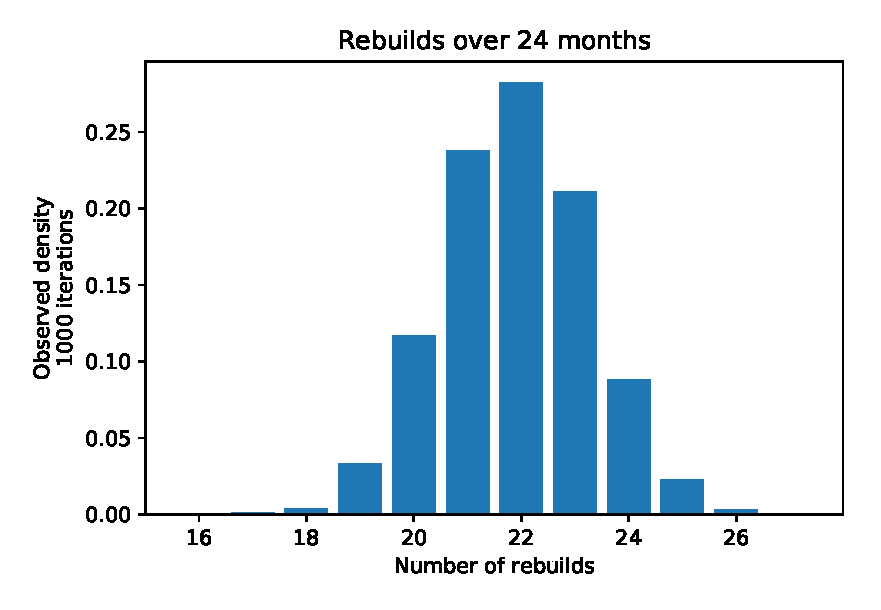
\includegraphics[scale=0.5]{RS-appendix-files/example_pmf.eps}
    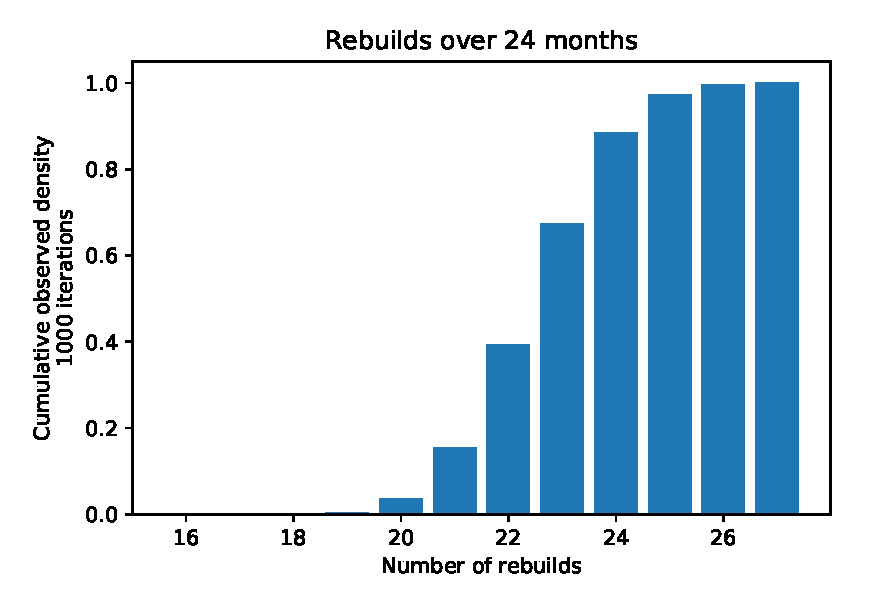
\includegraphics[scale=0.5]{RS-appendix-files/example_cdf.eps}
    \caption{Top: Density for the number of rebuilds over a 24 month period, repeated for 1000 iterations. Bottom: CDF of the number of rebuilds. In this case, the mean rebuilds/month value would be taken as $26/24\approx1.083$, with there being a 99.7\% chance that a file is rebuilt at most 26 times over the course of 24 months.}
    \label{fig:sim_method}
\end{figure}

\pagebreak
\linespread{1}
\pagebreak
\subsubsection{The decision tables}
In forming the decision tables, we consider as part of our calculations how
different choices of k, n, m, and mean time to failure affect durability and repair bandwidth. What we are looking for is the lowest repair bandwidth that also meets our
durability requirements.
\begin{table}[!htpb]\centering

\begin{tabular}{| c | c c c | c | c|}\hline
MTTF (months) &$k$& $n$ & $m$ &Repair Bandwidth Ratio&Durability (\# nines) \\\hline
1 &20& 40 & 35 & 9.36 & 0.9999 (8) \\
6 &20& 40 & 30 & 0.87 & 0.9999 (17) \\
12 &20& 40 & 25 & 0.31 & 0.9999 (13)\\\hline

1 &30& 60 & 35 & 3.40 &0.9999 (4)\\
6 &30& 70 & 40 & 0.60 &0.9999 (15)\\
12 &30& 80 & 45 & 0.31 &0.9999 (25) \\\hline

1 &40& 80 & 60 & 5.21 &0.9999 (4)\\
6 &40&120&50 & 0.52 &0.9999(14)\\
12 &40&120&45 & 0.24 &0.9999 (11)\\\hline

\end{tabular}
\caption{Decision tables showing the relationship between churn (MTTF),
  Reed-Solomon parameters ($k$, $n$, $m$), repair bandwidth ratio, and durability}
\label{rs:decision-tables}
\end{table}




\subsection{Making a decision}

We conclude by observing that these models may be tuned to target specific network scenarios and requirements. One network may require one set of Reed-Solomon parameters, while a different network may require another. In general, the closer $m/n$ is to 1, the more rebuilds per month should be expected under a fixed churn rate. While having a larger ratio for $m/n$ increases file durability for any given churn rate, it comes at the expense of more bandwidth used since repairs are triggered more often. To maintain a low mean rebuilds/month value while also maintaining a higher file durability, the aim should be to increase the value of $n$ as much as feasible given other network conditions (latency, download speed, etc.), which allows for a lower relative value of $r$ while still not jeopardizing file durability. 

Informally, it takes longer to lose more pieces under a given fixed network size and churn rate. Therefore, to maximize durability while minimizing repair bandwidth usage, $n$ should be as large as existing network conditions allow. This allows for a value of $m$ that is relatively closer to $k$, reducing the mean rebuilds/month value, which in turn lowers the amount of repair bandwidth used. 

For example, assume we have a network with a mean time to failure of six months.
Suppose we consider the same file encoded with two different RS parameters: 
one under a $(20,40)$ schema and the other as an $(30,80)$ schema. If we set $m$ so that $m=k+10$ for both cases, we observe from the above table
that the bandwidth repair ratio is is $0.87$ in the $(20,40)$ case and is $0.60$ in the $(40,80)$ case. Both encoding schemes have similar durability, as a repair in both cases is triggered when there are $k+10$ pieces left; even though, the mean rebuilds per month 
is empirically and theoretically lower for the $(40,80)$ case using $m=k+10$. 








\newpage \bibliographystyle{unsrt} \begingroup \raggedright
\bibliography{biblio} \endgroup

\end{document}
